% Introduction part II
This is the part of the report where the literature study will be presented. It starts by introducing general concepts related to game development, specifically how to design an enjoyable game, player types, and game reward systems. After that, an explanation of what an alternative game is, together with some common characteristics and a description of existing alternative games is described. Even though this content is a part of our contribution, it is included in this part because it is needed before discussing existing alternative games. At last, a technology review, discussing possibilities in the field of alternative games, is presented.
\clearpage

\documentclass[../Main.tex]{subfiles}
\begin{document}

\section{Design an Enjoyable Game}
\label{chap:designanenjoyable}
How to create an enjoyable game is an important part of every game development process. This chapter presents a literature study of the subject based on work conducted by \citeauthor{malone_what_1980} in \citeyear{malone_what_1980}, and \citeauthor{sweetser_gameflow_2005}’s “GameFlow: a model for evaluating player enjoyment in games” article. \citeauthor{malone_what_1980}’s research outlines challenge, fantasy, and curiosity as the three main elements increasing motivation in games. The GameFlow article presents a model for evaluating enjoyment in games based on eight elements. Even though different authors wrote these articles, they present a lot of the same mindset in what characterizes an enjoyable game.

\subsection{What makes things fun to learn?}
Malone presented in his study from \citeyear{malone_what_1980} a framework for creating enjoyable games. As mentioned above, he organized the essential elements of a good game into the three categories—challenge, fantasy, and curiosity. Malone wrote multiple articles on the topic. His main findings were summarized in “What Makes Things Fun to Learn? Heuristics for Designing Instructional Computer Games”. Even though this research was conducted in 1980 and the examples he presents are somewhat old, the main concepts are still highly relevant today.

\subsubsection{Challenge}
The first property presented by Malone is \textit{challenge}:

“In order for a computer game to be challenging, it must provide a goal whose attainment is uncertain.” \citep{malone_what_1980}. 

From this principle, three essential characteristics of why challenge is essential in good computer games follow:

\textbf{Goal} \\
As the first of the characteristics, goal is presented. Based on studies done by Malone, users tend to prefer games that have clearly defined goals. However, it is important to note that all goals are not equally valuable. Consequently, four different properties on how to create appropriate goals are mentioned:
\begin{enumerate}
    \item Simple games should include obvious goals.
    \item A complex environment should provide a structure so that players can easily generate appropriately difficult goals.
    \item Practical and fantasy goals are often the best ones.
    \item Players need to know when they are getting closer to the goal.
\end{enumerate}

\textbf{Uncertain outcome} \\
The next characteristic of how computer games can become challenging is an uncertain outcome. The article describes four different ways to achieve this:

\begin{enumerate}
    \item \textbf{Variable difficulty levels}\\ 
    Good computer games should include variable difficulty levels that can match the user’s skill level. The difficulty level can be determined in three ways: Automatically, chosen by the player, or determined by the opponent’s skills.

    \item \textbf{Multiple level goals} \\ 
    Finding a goal for various player types is easier when creating multiple level goals. Generally, two levels of goals are defined: Basic goals and meta goals. One typical example of this could be a primary goal of completing a level in a platform game. Collecting all the coins could then be the meta-goal. 

    \item \textbf{Hidden information} \\
    Hiding information can be an appropriate way of creating challenging games. Guessing games use this technique regularly. One example is Kriegspil, a variant of regular chess, where the players cannot see the opponent's board. This variant creates a new experience of playing chess, even though the game elements are the same.

    \item \textbf{Randomness} \\
    One last way of creating challenging games is to include randomness. When a random element is included, the player cannot predict the next step, hence making the game more challenging. Gambling games primarily succeed on the basis of randomness.
\end{enumerate}

\textbf{Self-esteem} \\
In addition to goals and uncertain outcomes, self-esteem is mentioned in the article. Self-esteem can be viewed as the reason why goals and challenges are essential in good games. Goals and challenges can increase a person’s self-esteem and thus create a captivating game. People often feel better about themselves when being successful in computer games, according to the article.

\subsubsection{Fantasy}
The next characteristic is fantasy, which is often used in games to make them more appealing. In games, fantasies often appear as models of physical objects and social settings that are not truly present. Also, there may be situations or objects in these fantasies with varying degrees of impossibility, varying from absolutely impossible to utterly possible \citep{malone_what_1980-1}.

In learning games, one can increase the fun by overlaying the curriculum with elements of fantasy. The fantasy can visualize the progression of the player towards the goal based on right or wrong answers. The goal may be to achieve a fantasy goal, like getting to the finish line in a marathon, or it may be avoiding some catastrophe, like the man getting hung in Hangman. In these games, the fantasy depends on how the skill is used, but not necessarily vice versa. Fantasies that only have the one-way logical dependency, where skill affects the fantasy, is called extrinsic fantasies. Extrinsic fantasies are good for arithmetic problems, where answers are either wrong or right, and the skill does not depend on the fantasy  \citep{malone_what_1980}.

\begin{figure}[H]
    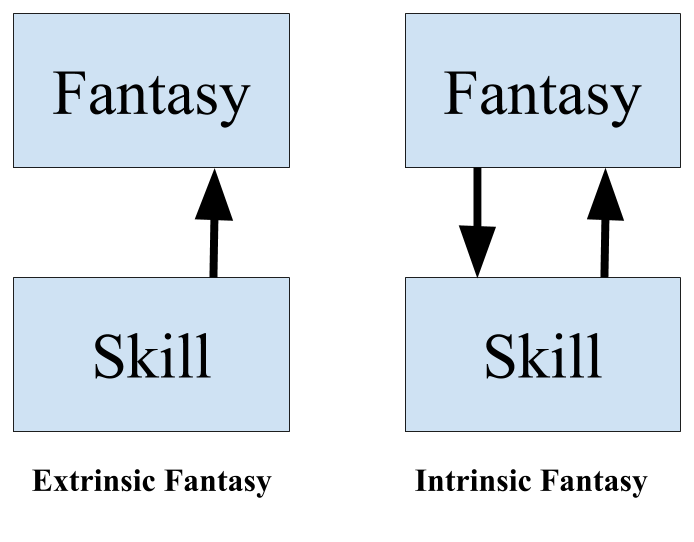
\includegraphics[width=0.5\textwidth]{Images/Theory/SkillFantasy.png}
    \centering
    \caption{Logical dependencies in extrinsic and intrinsic fantasies\citep{malone_what_1980}.}
    \label{fig:skill_fantasy}
\end{figure}

Fantasies that have a two-way logical dependency are called intrinsic fantasies; the fantasy depends on the skill, and the skill depends on the fantasy. Figure \ref{fig:skill_fantasy} illustrates the two types of fantasy side-by-side. In the spelling game Hangman, the player’s spelling skills affect the fantasy, and the feedback of right or wrong guesses from the fantasy influences the player's skill as it becomes easier to guess new letters each time. Malone (\citeyear{malone_what_1980-1}) stated, “intrinsic fantasies are both more interesting and more instructional than extrinsic fantasies,” and it seems to be true for various reasons. One reason being that the use of skill in intrinsic fantasies often can be applied to real-world situations,like the game Lemonade Stand mentioned by Malone in his \citeyear{malone_what_1980-1} dissertation. In an audio-only version of the game, found on Amazon Alexa, children have to use their pre-existing knowledge and skills to sell lemonade \citep{einhorn_amazoncom_2019}. For this particular game, children may train their skills to handle money and do maths and later apply it to real-world situations. Malone further argues that when fantasies are closely related to the curriculum, they can use their existing knowledge to exploit analogies between what they know and the material. Building new knowledge and skills from pre-existing knowledge relates to the cognitive aspect of fantasy. In Lemonade Stand, players have to apply what they know of the physical objects involved in a lemonade sale, e.g., Lemons and money. If they connect product cost and price, or weather and sales, they will improve their maths, money, carefully listening, business, and probability.

\textbf{The emotional aspect of fantasy} \\
Fantasies in games can appeal to players differently based on what emotions they need to satisfy \citep{malone_what_1980-1}. It may be challenging to design a computer game that meets the emotional needs of the person playing. Lazzaro stated in (2008) that emotions are the key to a great player experience (PX), and game designers cannot directly design player emotions. However, they can design rules for choices and feedback, so-called mechanics. Mechanics are used to triggering certain emotions that engage and motivate players \citep{lazzaro_four_2008}. Lazzaro’s studies are partly based on Malones \citeyear{malone_heuristics_1982} conference paper, where he discusses how fantasy affects motivations. He states that “... fantasies can be very important in creating intrinsically motivating environments but that, unless the fantasies are carefully chosen to appeal to the target audience, they may actually make the environment less interesting rather than more.” \citep{malone_heuristics_1982}. This statement suggests that different people find different fantasies appealing and that the fantasy must be appropriate for the target audience. Furthermore, if games had different fantasies to choose between, players are more likely to find it enjoyable, motivating, and engaging, because it has a broader appeal.

\subsubsection{Curiosity}
The last characteristic, curiosity, is about a player’s motivation to learn within a game environment. The learning is, however, independent from goal-seeking or fantasy-fulfillment. Games can trigger a player's curiosity by creating environments that have optimal information complexity. This implies that the environment must not have too high, nor too low, information complexity regarding the player’s existing knowledge. Finding such balance for the information complexity will evoke the player’s curiosity to explore the environment further. An optimal environment has a complexity level where the player uses its knowledge to create an expectation of how the environment should behave. Still, these expectations should sometimes be unmet to be novel and introduce an element of surprise.

Malone states that there are two characteristics in the category that should be distinguished: sensory curiosity and cognitive curiosity.

\textbf{Sensory curiosity} \\
Sensory curiosity is about the use of sensory-stimulating technology that attracts the user’s attention. Sensory curiosity is not only used in games; it can also be found in movies and TV shows as change or patterns in light, image, audio, or other sensory stimuli. In games, sensory curiosity appears as both audio or visual effects. Malone goes on to suggest that the effects can be used in four main ways. These usages can also appeal to other motivations than curiosity \citep{malone_what_1980}.

\begin{enumerate}
    \item \textbf{As decoration} \\
    The use of audio and visual effects that are present regardless of user interactions. In games like Just Dance Now, this can be found as background music in the menu. Malone states that effects like in-game background music may initially increase the player’s interest, but it will quickly become tiresome. 
    \item \textbf{For enhancing fantasy} \\
     It is used to enhance fantasy in a game like “decorative” effects. However, the special effects are distinguishable because of its captivating nature and association with the fantasy. In Wii Fit, this appears as audio effects that mimic an audience. Not only does this enhance the fantasy, but it also strengthens the immersion in the game.
    \item \textbf{As a reward} \\
    The use of audio and graphical effects to reward good performance. It can increase the motivation for reaching the goal. Pokémon Go uses flashing lights and stars, together with victory sound, when users perform well, for instance, when they catch a new Pokémon. However, the challenge related to reaching a defined goal can shift the focus away from users exercising their curiosity. 
    \item \textbf{As a representation system} \\
    Is the use of audio and visuals to convey information without using text. This usage is widely used in games to convey information to the user efficiently. If a player in Pokémon Go unsuccessfully throws a Pokéball at a Pokémon, then the Pokéball will bounce away to indicate that a player missed the Pokémon.  
\end{enumerate}

\textbf{Cognitive curiosity} \\
Cognitive curiosity is about the desire to improve one’s knowledge structures. Malone claims that people prefer their cognitive structures to be complete, consistent, and parsimonious. According to his theory, to stimulate a player’s cognitive curiosity, they must be given just enough information to make their existing knowledge appear incomplete, inconsistent, or unparsimonious. This will engage the user because people are willing to learn more to improve their knowledge-structures. For instance, if a person only has 10 minutes left of a movie, they will likely finish the film to bring completeness to their knowledge structure.

These general ideas are the root of several game design principles. One way is to produce responsive feedback that makes environments more interesting. Malone then goes on to present two-game design ideas about informative feedback.

\begin{itemize}
    \item \textbf{To engage a learner’s curiosity, feedback should be surprising.} \\
    Surprising feedback can simply be random feedback that relates to the subject. Another way to have surprising feedback in the environment is to have an underlying consistency that is not clear at first. 
    \item \textbf{To be educational, feedback should be constructive.} \\
    Constructive feedback should not only reveal if applied knowledge is incomplete, inconsistent, or unparsimonious; it should also indicate how the user can improve their input to become complete, consistent, and parsimonious.
\end{itemize}

\subsection{GameFlow}
Another essential framework for creating good games is Sweetser and Wyeth’s GameFlow (2005). The authors define a model for designing, evaluating, and understanding enjoyment in games based on work previously done by \citeauthor{csikszentmihalyi_flow_1990} in 1990. \citeauthor{csikszentmihalyi_flow_1990} conducted extensive research and surveys to find out what makes experiences enjoyable. Sweetser and Wyeth modified these principles to be representative of enjoyment in games. The GameFlow model consists of eight elements—concentration, challenge, skills, control, clear goals, feedback, immersion, and social interaction. Each of these includes a goal and a set of criteria that can be used when developing games \citep{sweetser_gameflow_2005}.

\subsubsection{Concentration}
Concentration is the first of the eight elements presented in the article. Enhancing how much concentration a task requires increases its immersion. Games should grab the player’s attention immediately and keep holding it for as long as possible. The player’s workload should be maintained at an appropriate level, and unimportant tasks should not be presented during the game to achieve this. Also, nongame-related interactions (e.g., settings menu) should be minimized, and the game should strive to use as much screen as possible for the gameplay. 

In Guitar Hero, players have to stay highly concentrated throughout the game. The gameplay is set in an environment with little distractions so that the player can become more immersed. The game also forces the player to stay concentrated throughout the song, not to reach the game-over state. Figure \ref{fig:guitar_hero_gameplay} illustrate a screenshot from the gameplay in Guitar Hero.

\begin{figure}[H]
    
\includegraphics[width=0.8\textwidth]{Images/Theory/GuitarHeroGameplay.jpg}
    \centering
    \caption{Screenshot of gameplay in Guitar Hero.}
    \label{fig:guitar_hero_gameplay}
\end{figure}

\subsubsection{Challenge}
Challenge is often considered the essential aspect of good game design, and appropriate challenges should be presented to the player. The players’ skill levels should match the challenges given. Additionally, the challenge level should increase as the player moves through the game at an appropriate pace. In the language learning game Duolingo, players take a placement test to start at an appropriate level of challenge, as seen in Figure \ref{fig:dulingo_placement_test}.

\begin{figure}[H]
    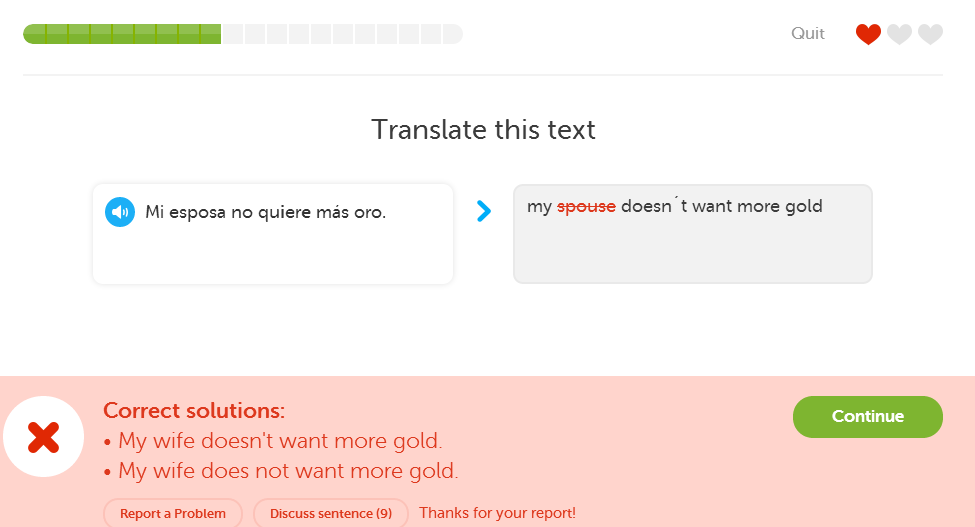
\includegraphics[width=0.7\textwidth]{Images/Theory/DuolingoPlacementTest.png}
    \centering
    \caption{Spanish placement test in Duolingo.}
    \label{fig:dulingo_placement_test}
\end{figure}

\subsubsection{Player Skills}
As mentioned above, the player’s skill level needs to match the difficulty level of the game. The player’s skills also need to increase during the game at the same rate as the difficulty of challenges so that the game does not get too difficult (or too easy). Rewarding players appropriately when completing specific tasks, with points or similar, is an essential part of this process.

Again, in Duolingo, players are matched with the appropriate skill level, and as the game progresses, both the player’s skills and the level of difficulty grows. The placement test, in Figure \ref{fig:dulingo_placement_test}, makes sure that players are met with an appropriate level of difficulty. Also, players have to put their knowledge to the test before they are allowed to ascend to the next level. This additional test mechanism makes sure that users are qualified for new levels and prevents players from being demotivated from challenges that are too demanding.

Furthermore, the player needs to manage to start the game without reading the manual, and learning how to play should not be boring. Explanations during the initial levels or a tutorial that replicates playing the actual game are examples of how learning the game can be fun. If the user needs additional help, an online manual should be available. This prevents the player from exiting the game when not knowing what to do.

\subsubsection{Control}
Another central element of good game design is control. The players should feel a sense of control over their actions in the game and be able to transfer their intentions to in-game behavior. Essential aspects of the game to achieve this are good interfaces and easy to use input devices. Controlling the game should be intuitive and straightforward. Also, the players should feel in control of their actions and strategies and play the game the way they want. In addition to this, players should not make errors that are disturbing to the gameplay. If they do, recovering from errors should be supported. 

Racing games are, in general, examples of games that are intuitive to maneuver. Custom racing wheel controllers mimic the action of actually driving a car, as seen in Figure \ref{fig:racing_wheel_controller}. Recovering from errors that are disturbing for the gameplay, such as flipping the car or driving off a cliff, is also usually supported with a “reset” button.

\begin{figure}[H]
    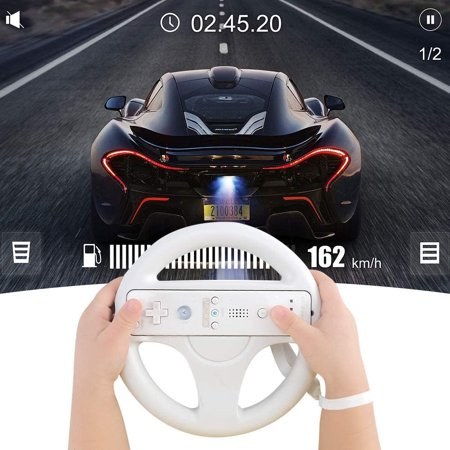
\includegraphics[width=0.5\textwidth]{Images/Theory/wii_racing_wheel_control.jpeg}
    \centering
    \caption{ Wii Steering wheel used when playing a racing game.}
    \label{fig:racing_wheel_controller}
\end{figure}

\subsubsection{Clear Goals}
Clear goals should be provided to the user at appropriate times. A primary goal should initially be presented to the user. Some introductory cinematic background that tells the background of the story is often used to describe this goal to the user. Intermediary goals should be provided to the user when they progress. Games often use “briefings” or “missions” for this. 

In Super Mario Bros, players are introduced to a mission of saving Princess Peach from the villain Bowser. This background establishes a clear goal for the entire game. The game also has intermediate goals of completing each level towards the final goal.

\subsubsection{Immersion}
Immersion describes a deep and effortless involvement in games. Players should feel engaged by the game so that they may experience an altered sense of time, less awareness of surroundings, less self-awareness, and fewer worries. Immersion also indicates emotional attachment to the game.

Deep and effortless involvement in games is often presented in studies of game-players \citep{johnson_effective_2003}. People play games to “escape” from the real world. Essential aspects of improving the immersion of a game are audio and narratives. Sounds and music in games improve the players’ attraction to the game and keep them immersed for a more extended period. A story or narrative that gives the player some background information or a storyline to follow also creates the same effect.

\begin{figure}[H]
    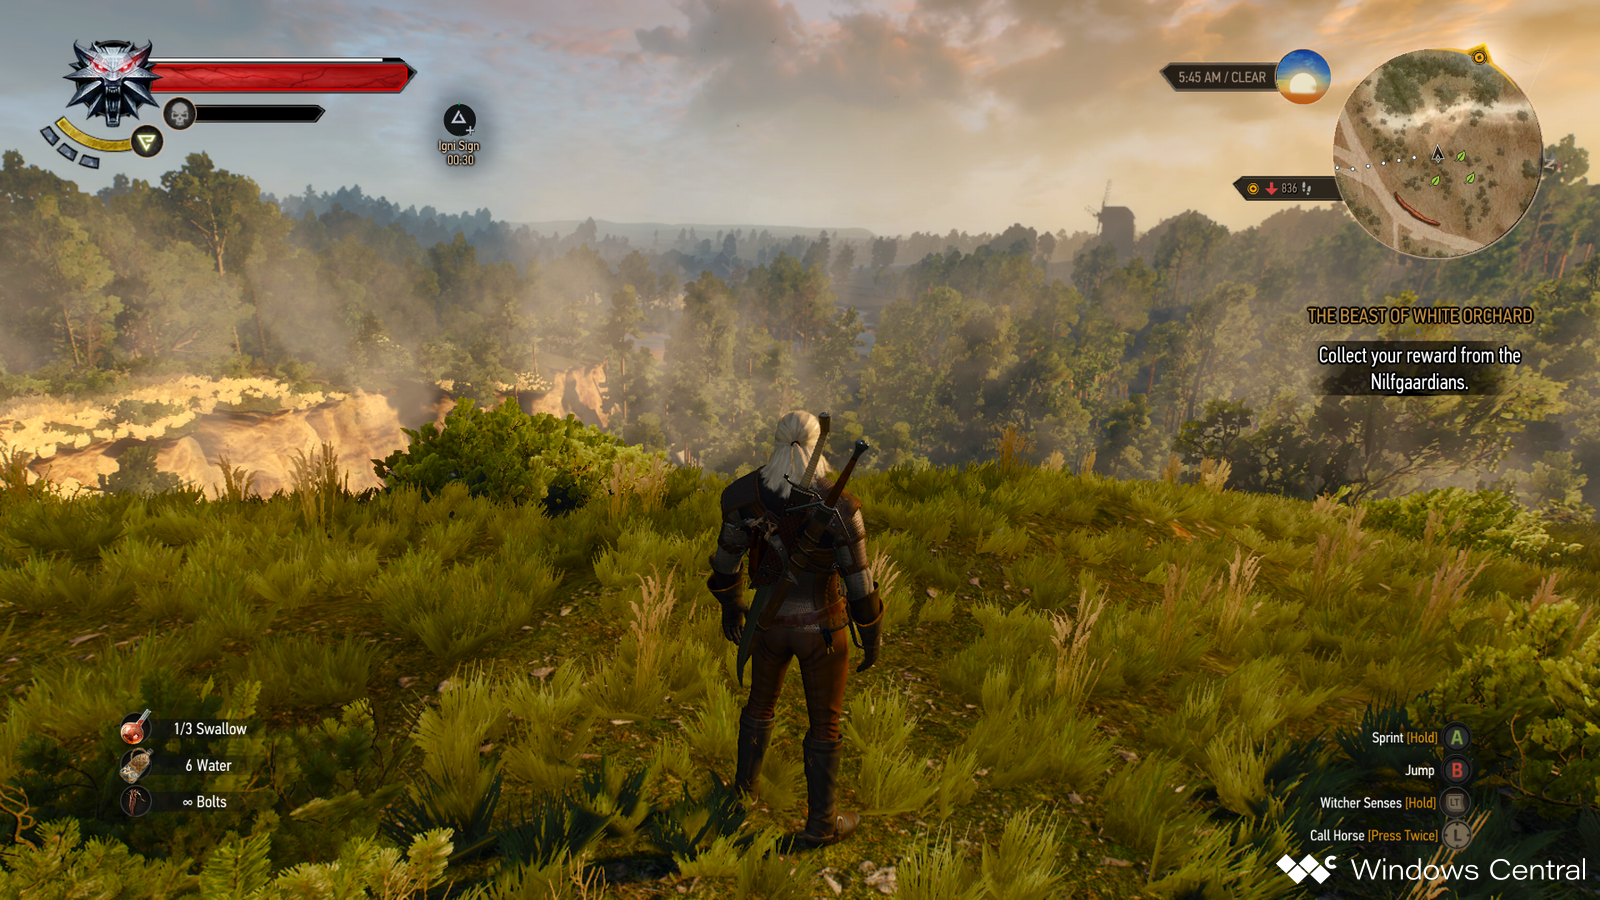
\includegraphics[width=0.8\textwidth]{Images/Theory/witcher3_immersion.png}
    \centering
    \caption{Gameplay screenshot from Witcher 3.}
    \label{fig:witcher3_immersion}
\end{figure}

The role-playing game the Witcher 3 has become known for being a highly immersive open-world game. The game has a strong storyline, realistic graphics and audio, and many intermediate goals that draw the player deeper into the game, as seen in Figure \ref{fig:witcher3_immersion}. For the Witcher 3, immersion can cause players to feel an emotional attachment to the game and reduced concern for self and sense of time.

\subsubsection{Feedback}
\begin{wrapfigure}{r}{0.4\textwidth}
    \centering
    \vspace*{-2.5\baselineskip}
    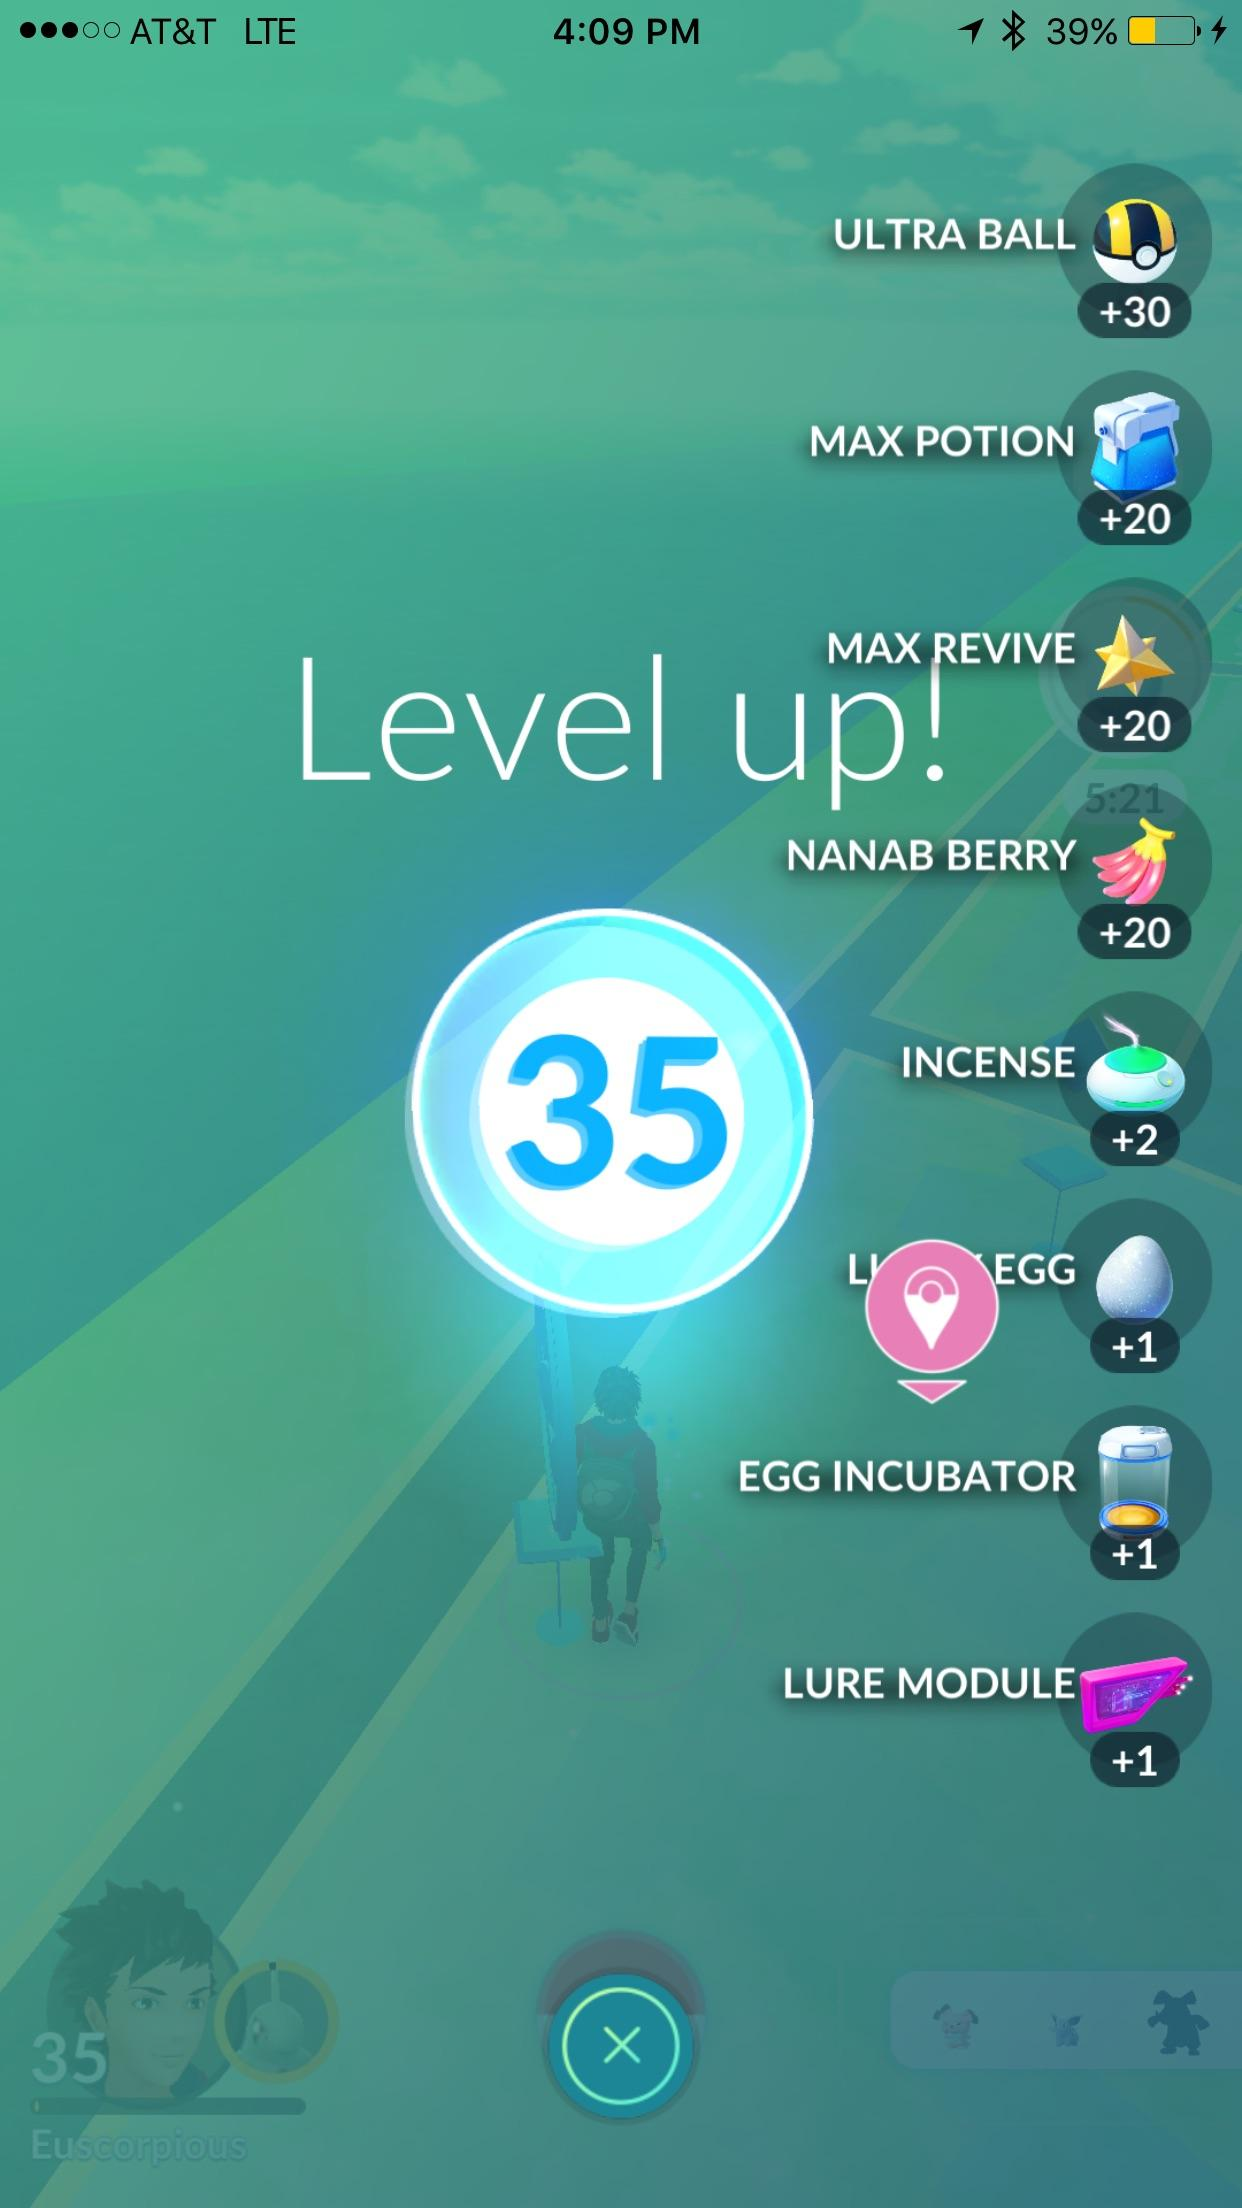
\includegraphics[width=0.3\textwidth]{Images/Theory/PokemonGoLevelUp.jpg}
    \caption{Feedback in Pokémon Go when leveling up.}
    \label{fig:pokemon_go_level_up}
\end{wrapfigure}

Players should get the feedback they need during the game. They should always know their status or score and progress towards the goal. Additionally, appropriate feedback should be provided on their actions. 

Pokémon Go uses direct and immediate feedback. Visual, textual, and audio feedback is used frequently. The game also uses points, levels, streaks, and medals to award good performance and engagement. Figure \ref{fig:pokemon_go_level_up} show the visual feedback a player receives when leveling up in Pokémon Go. 

%\begin{figure}[H]
   % 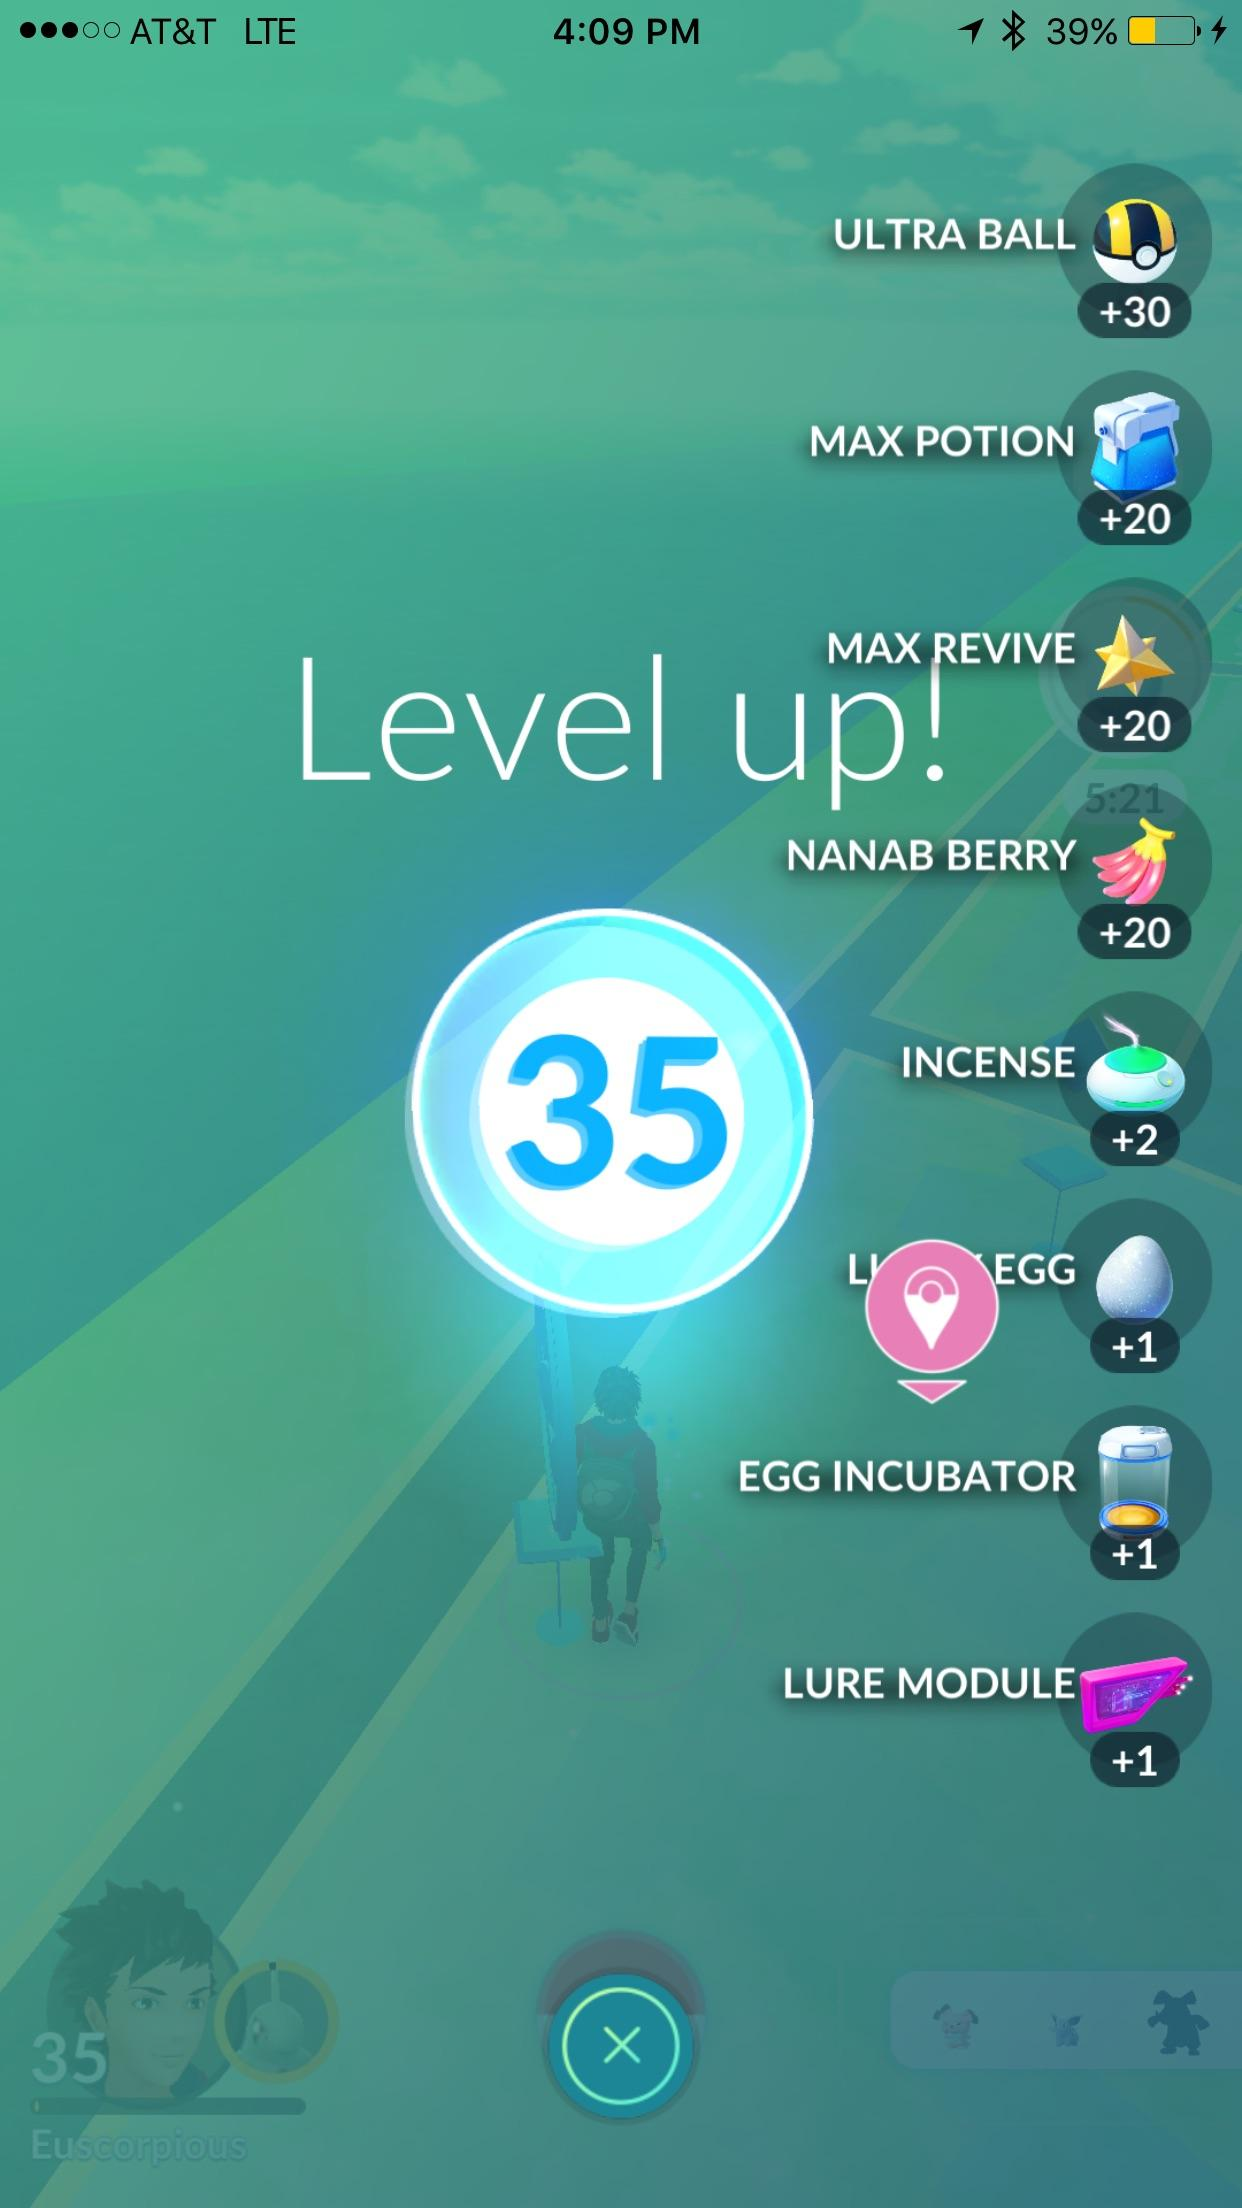
\includegraphics[width=0.5\textwidth]{Images/Theory/PokemonGoLevelUp.jpg}
   % \centering
   % \caption{Feedback in Pokémon Go when leveling up.}
   % \label{fig:pokemon_go_level_up}
%\end{figure}


\subsubsection{Social Interaction}
The last element in the GameFlow model is not an element of flow. Social interaction may often interrupt the immersion in games. However, it is an important element in the GameFlow model because social interactions improve enjoyment in games. Games should support and create opportunities for player-to-player interaction and social competitions. Online games are a typical example of how important social interaction can be. In this type of game, social interaction is often the main reason people are attracted to them. World of Warcraft is a classic example of such a game.

\subsection{Summary}
In this chapter, two frameworks describing how to create an enjoyable game have been presented. The frameworks include a description of central characteristics in game-design related to creating good games. Even though all the characteristics presented in the frameworks are essential aspects of game design, every game should not necessarily include all of them. As a game developer, the important task is to know about theory and utilize the appropriate parts of it.

As with the development of most games, an alternative game’s success depends on which degree the game is enjoyable for the user. How captivating and fun is the game? The design of our game will use characteristics from the theory presented in this article.

\biblio % Needed for referencing to working when compiling individual subfiles - Do not remove
\end{document}
\clearpage

\documentclass[../Main.tex]{subfiles}
\begin{document}

\section{Player types}
\label{chap:playertypes}

Players can have very different interests for playing. Consequently, it is therefore important to consider these interests when designing games. This chapter present \citeauthor{hamari_player_2014}(\citeyear{hamari_player_2014}) on player types

\citet{bartle_hearts_1996}

\biblio % Needed for referencing to working when compiling individual subfiles - Do not remove
\end{document}
\clearpage

\documentclass[../Main.tex]{subfiles}
\begin{document}

\section{Reward Systems}
\label{chap:rewardsystems}


\biblio % Needed for referencing to working when compiling individual subfiles - Do not remove
\end{document}
\clearpage

\documentclass[../Main.tex]{subfiles}
\begin{document}

\section{What is an Alternative Game?}
\label{chap:what_is_alternative}
To develop a concept for an alternative game (as described in the research goal), a clear understanding of which games can be categorized as alternative games is crucial. Let us first take a look at what the word “alternative” means in this context with some definitions from three well-known dictionaries:

\blockquote{
    \textit{“Different from the usual or traditional way in which something is done”} \\
    \textbf{Oxford learner's dictionary}
    
    \textit{“Different from the usual or conventional”} \\
    \textbf{Merriam-Webster's Collegiate Dictionary}
     
    \textit{“Alternative things are considered to be unusual and often have a small but enthusiastic group of people who support them”} \\
    \textbf{Cambridge dictionary}
}

While all of these dictionaries define the word differently, we can see that there are some commonalities. All three describe alternative as something “unusual” or “different from the usual.” The key takeaway from the definitions is that an alternative game is a game where the creators have done something in such a way that it differs from ordinary games.

To recognize alternative game concepts more easily, we will examine existing alternative games and analyze what they have in common. The result of this research is a list of six characteristics, where alternative games often differ from ordinary ones.

\subsection{Alternative Game Characteristics}
Our proposal of which games can be considered alternative games is then the following:

\textit{If a game deviates from regular games in one or more of the game characteristics categories mentioned in this chapter, it can be considered an alternative game.}

Below are explanations of all categories with coherent, relevant alternative games presented. These categories are covering all alternative games we have studied during this phase of the project. However, it is important to point out that there might exist additional characteristics from games that we are not aware of or that are not developed yet. As technology moves forward, it is reasonable to assume that new branches of alternative games might emerge.

\subsubsection{Input}
A common way of creating an alternative game is to use an unusual input source (such as the GPS, microphone, special controllers, or accelerometer) for controlling the game. Three examples of games using alternative input sources are Knowledge War \citep{wang_knowledge_2016}, CityZombie \citep{zhu_experiences_2010} and Exermon \citep{wang_evaluation_2017}. Both Knowledge War and CityZombie use the user’s position as a central part of playing the game. Moving around in the real world translates to the gameplay. Exermon is an example of utilizing the accelerometer on the player's phone. The game is a strength-based exercise game that tries to motivate people to do more strength exercises. An alternative input source, the accelerometer, is used to register the number of repetitions the user completes in one workout.

\subsubsection{Output}
The output from the game is another characteristic commonly explored in the development of alternative games. Some known examples are sound, haptics, and augmented reality, but there are many more. Two examples of games using alternative outputs are “Unexceptional.net” and “The Amazing City Game.” Unexceptional.net is a story-driven pervasive game where “the story evolves through multiple media channels interacting with the player.” The game includes different untraditional outputs, such as SMS and phone calls, to provide feedback to the player \citep{wang_unexceptionalnet_2009}. The Amazing City Game is also a pervasive game where the players can play a knowledge competition tour. The game utilizes location and augmented reality to show different vital landmarks at a user’s location \citep{wang_pervasive_2011}.

\subsubsection{Target Group}
The target group is an essential characteristic of a game, and it decides what type of users the game should appeal to. Some games include adjustments to target specific groups of people, and some of these can make the game fall into the alternative game definition. More special target groups, like people with physical disabilities, often require more adjustments to play games at all. For example, people who cannot maneuver a game using traditional handheld controllers require other ways to interact. A Brain-Computer Interface (BCI) could be a way of bringing games to this group of people. One concrete example is the use of brain waves (via a \href{www.neurosky.com}{NeuroSky} brain set) to control the movement in a Snake game \citep{wang_using_2012}.

\subsubsection{Game Genre}
Computer games are generally categorized as one of eight game genres \citep{prensky_fun_2001}:

\begin{itemize}
    \item Action Games
    \item Adventure Games
    \item Fighting Games
    \item Puzzle Games
    \item Role-Playing Games (RPG)
    \item Simulation Games
    \item Sports Games
    \item Strategy Games
\end{itemize}

Earlier computer games were usually limited to one category, while today, games often fall into multiple ones. Additional categories may also be defined for games that do not directly belong to any of these genres. Alternative games often consist of unique concepts and uncommon gameplay, often falling into other categories than those mentioned above. An example of such a genre is gamification, defined as “the application of game design principles in non-gaming contexts” \cite{robson_is_2015}. The “Kinect Recycling Game” is an example of a game that do not fit directly into any of the eight general game genre categories. This game is a gamification concept of recycling trash, where the goal is to teach recycling in an engaging and realistic way. As the name implies, the game uses Kinect to recognize players' hand gestures to place the trash into the right bins \citep{wang_learning_2015}.

\subsubsection{Domain}
Computer games can be applied to different domains. The domain of a game depends on what area of use it serves. Some examples of game domains are entertainment, education, industry, government, and health. Alternative games may sometimes define their area of use, where the new domain may be a combination of other domains or a subset of an existing domain. For instance, edutainment games are a crossing between education and entertainment. Another example of an alternative domain is Attensi’s system for gamified work training, mixing industry, and learning \citep{attensi_why_2020}. The company offers tailored 3D job simulators to large organizations to achieve real and measurable changes in employees’ behavior and skills.

\subsubsection{Interaction}
There exists a lot of various interaction forms for games. Examples included cooperation, competition, player vs. player (PVP), and more. Interaction can also contain an alternative twist, i.e., interaction forms that are not used in ordinary games. One such concept is the multimodal “Multiplayer On One Screen Entertainment System (MOOSES)” approach. Here, the players use their smartphones as controllers for gaming on a shared screen \citep{wang_evaluation_2010}. \href{http://www.airconsole.com}{AirConsole} is a concrete example of where this concept is utilized. The console includes multiple MOOSES based games where the players use their smartphones as controllers. Games can also be pervasive, meaning the game experience is extended beyond the fictive world. The player interacts with both the virtual and real worlds.

\subsection{Model}
Based on these six characteristics, we have created a model to help us compare alternative game concepts. Table \ref{tab:example_model} illustrates an example of how the model can look like for three fictional ideas, idea 1, idea 2, and idea 3. Each category includes characteristics relevant to the ideas compared. As an example in Table \ref{tab:example_model} shows, the ideas use GPS, Bluetooth, camera, gyroscope, and accelerometer as input. Idea 1 uses all of them, except Bluetooth, while idea 3 uses GPS and Bluetooth.

The model simplifies the comparison process of alternative games and justifies why the concepts can be categorized as alternative games. Thus, the model will be useful in both the description of existing alternative games in Chapter \ref{chap:existing_games} and the description of new ideas in Chapter \ref{chap:ideas}.

In addition to categorizing and defining alternative game concepts, the model can help us invent new ones by exploring the characteristics. Modifying different characteristics may create concepts that would otherwise not have been invented. Additionally, the model could increase the structure of a typical brainstorming session, by examining one characteristic at a time.

\begin{table}[H]
    \centering
    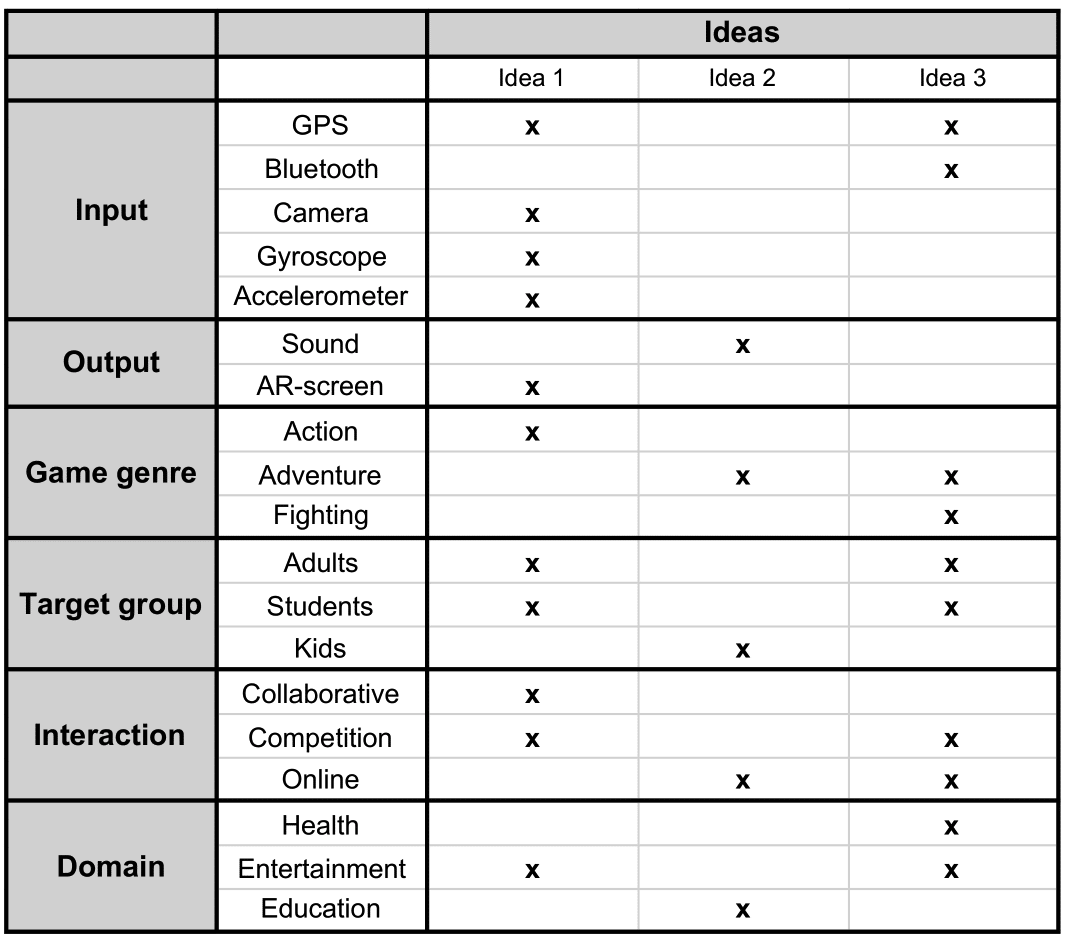
\includegraphics[width=0.75\textwidth]{Images/Models/ExampleModel.png}
    \caption{Categorizing alternative games, example model}
    \label{tab:example_model}
\end{table}

\subsection{Summary}
This chapter presented our definition of alternative games together with the six coherent categories of game characteristics. A short description of each of them with relevant examples from the literature was given. In the next chapter, existing popular and known alternative games will be described. How they fit into the proposed categories in this chapter will also be outlined.

\biblio % Needed for referencing to working when compiling individual subfiles - Do not remove
\end{document}
\clearpage

\documentclass[../Main.tex]{subfiles}
\begin{document}

\section{Existing Alternative Games}
\label{chap:existing_games}
In this chapter, seven different alternative games will be presented. The games are picked based on popularity, relevance today, and how they compare to each other. Different types of games are carefully chosen to illustrate the diversity of alternative games that exist. A brief explanation of the game concept and why it is an alternative game will be given in every game section.

\subsection{Hold}
Hold is an application that rewards users for not using their phones \citep{hold_hold_2020}. The game was initially launched in 2016 for iOS and Android, and the primary focus was on Norwegian university students \citep{ringheim_smarttelefon_2018}. Since then, the application’s target group has expanded beyond Norwegian students.

\begin{figure}[H]
    \begin{minipage}{.5\textwidth}
      \centering
      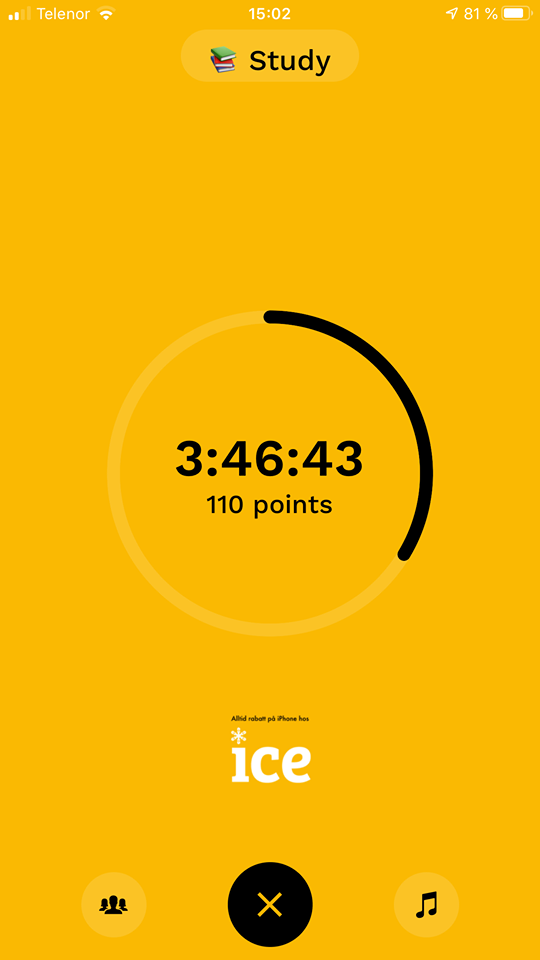
\includegraphics[width=.75\textwidth]{Images/ExistingGames/HoldApp.png}
      \captionof{figure}{Main timer screen in Hold.}
      \label{fig:hold_timer}
    \end{minipage}
    \begin{minipage}{.5\textwidth}
      \centering
      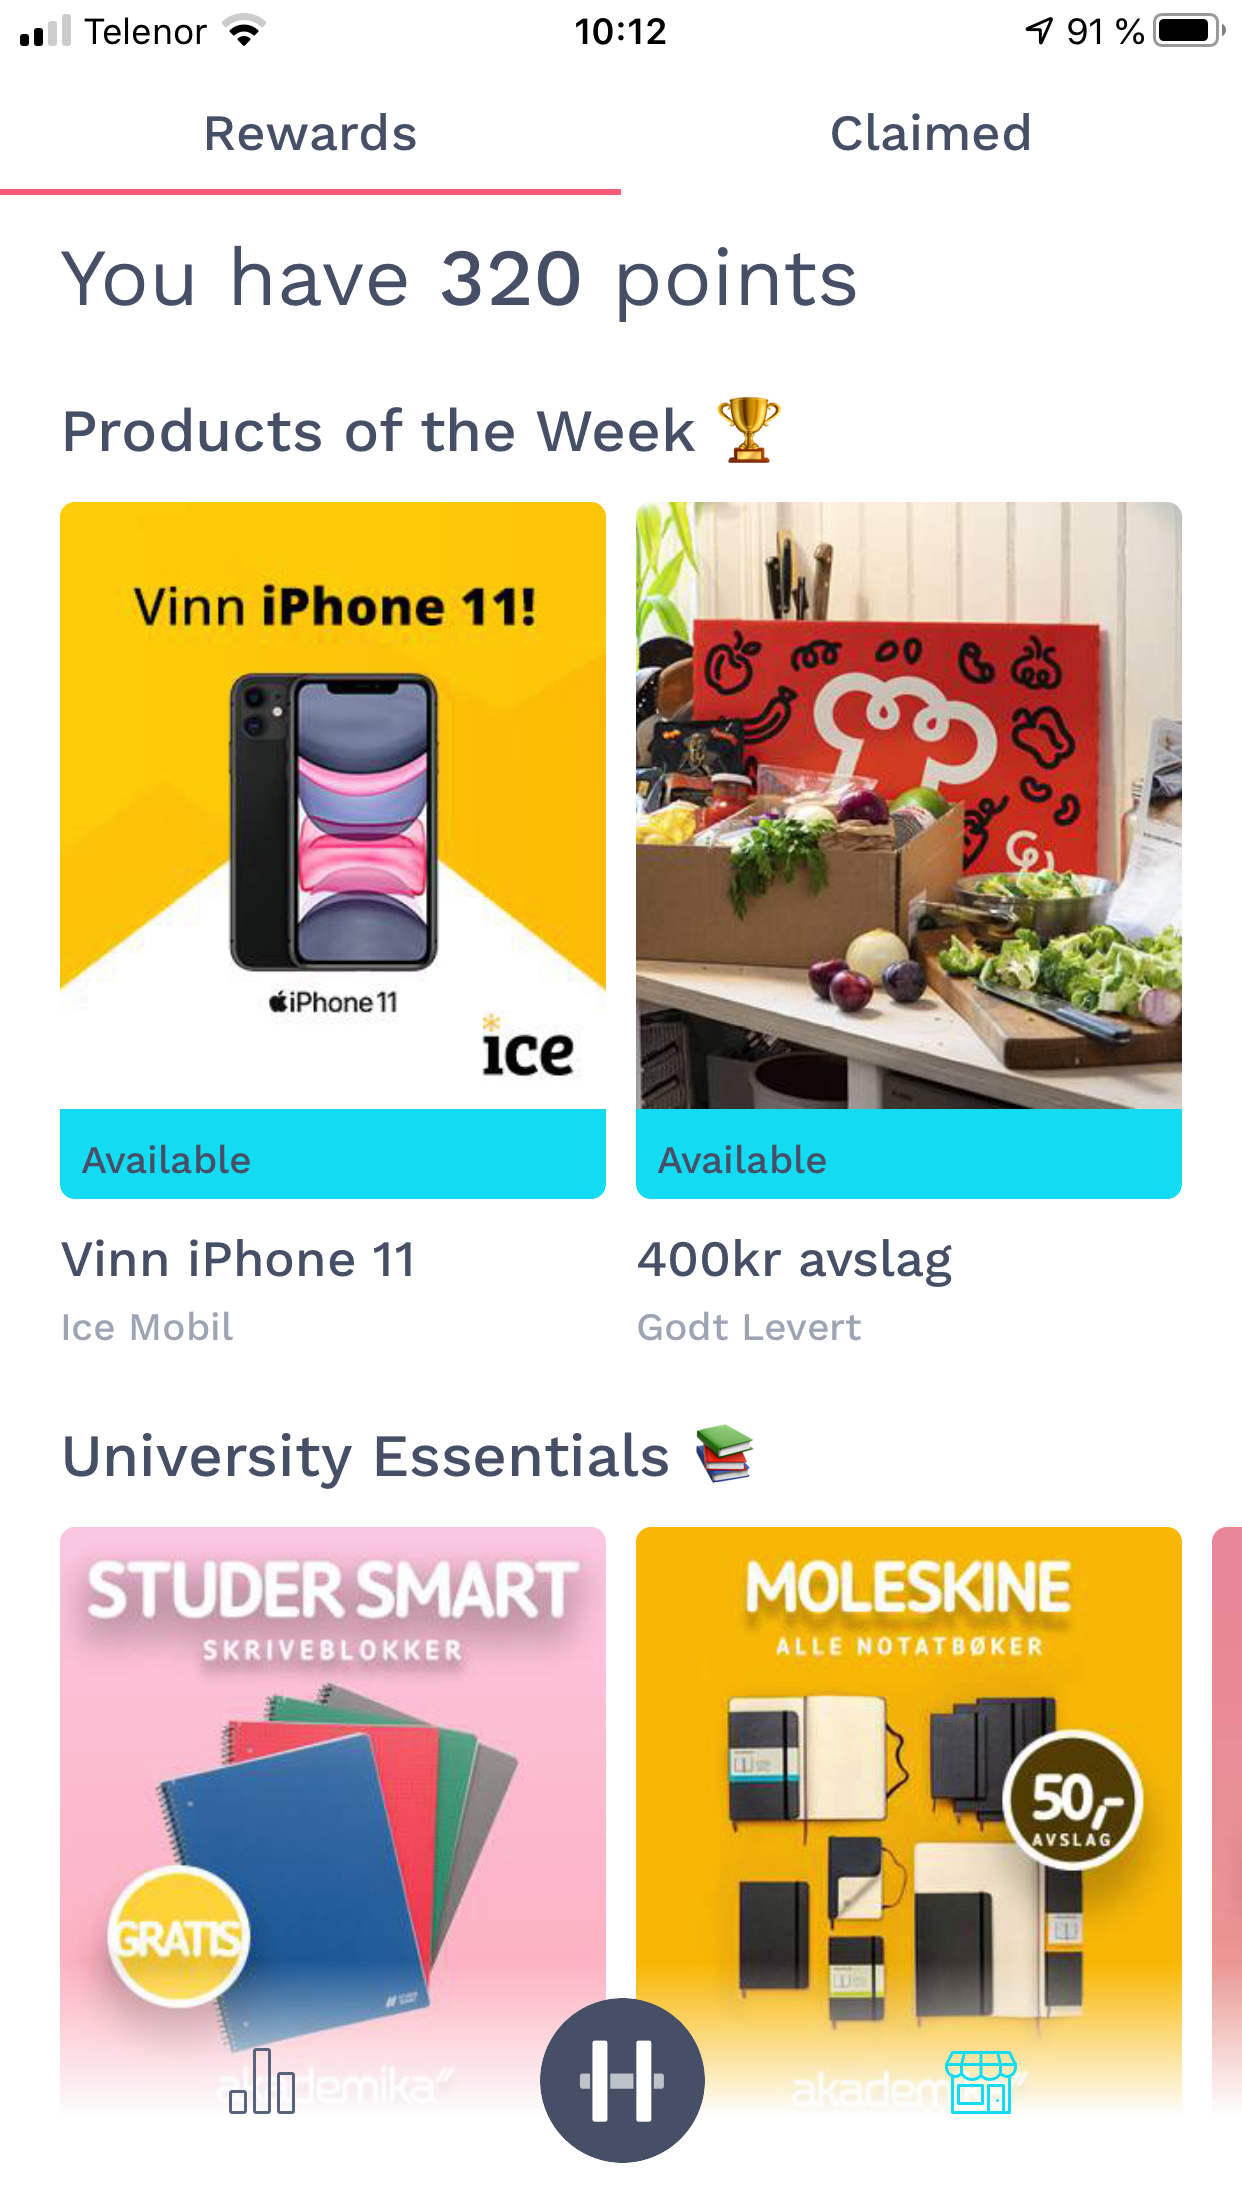
\includegraphics[width=.75\textwidth]{Images/ExistingGames/HoldAppRewards.png}
      \captionof{figure}{Choices of rewards in Hold.}
      \label{fig:hold_reward}
    \end{minipage}
\end{figure}

The application helps users limit distractions through gamification. When users activate the application, a timer starts running (see Figure \ref{fig:hold_timer}). The user is rewarded with ten points for each twentieth minute they are not using their phone. The points can later be exchanged into real-life items such as coffee, food, or discounts, as seen in Figure \ref{fig:hold_reward}. The rewards are the main motivating factor for using the application.

Unlike other games, Hold’s concept is to encourage people not to use their mobile phones. The user can choose to play alone against the environment (PvE) or connect with friends to compare scores, making it more of a competitive game (PvP). The application also lets users connect with nearby friends through Bluetooth, enabling them to focus (collaborate) while boosting their points collectively\citep{wakefield_free_2018}.

Hold is a perfect example of an alternative game with a different concept, where the developers have explored multiple of the game characteristics categories. The game classifies as an alternative primarily for two reasons: It explores alternative game genres by using gamification, rewarding the user points for not using their phone. Furthermore, it uses alternative input sources, primarily Bluetooth, for connecting with nearby friends.

\subsection{Mario Kart Live}
Mario Kart Live is a newly developed augmented reality concept from Nintendo (released 16th October 2020) for its Switch game console. The game is based on the classic Mario Kart game, but with a unique twist: the inclusion of a specially designed racing kart that follows the user’s maneuvers in-game. A live video feed from the racing kart is relayed to the user’s Switch, mapping the virtual track to the user’s home \citep{velazco_race_2020}. The game can be played individually (against AIs) or as a multiplayer game with more than one kart \citep{hashimoto_mario_2020}.

The game is a typical example of how the use of alternative sources for input and output can bring something new to an already familiar game concept. For this Mario Kart game, the alternative twist is the use of a camera for input to produce AR output. Figure \ref{fig:mario_kart_live} shows a poster from the game where you can see the karts racing a user’s home and how the game is presented to the player. 

\begin{figure}[H]
    \centering
    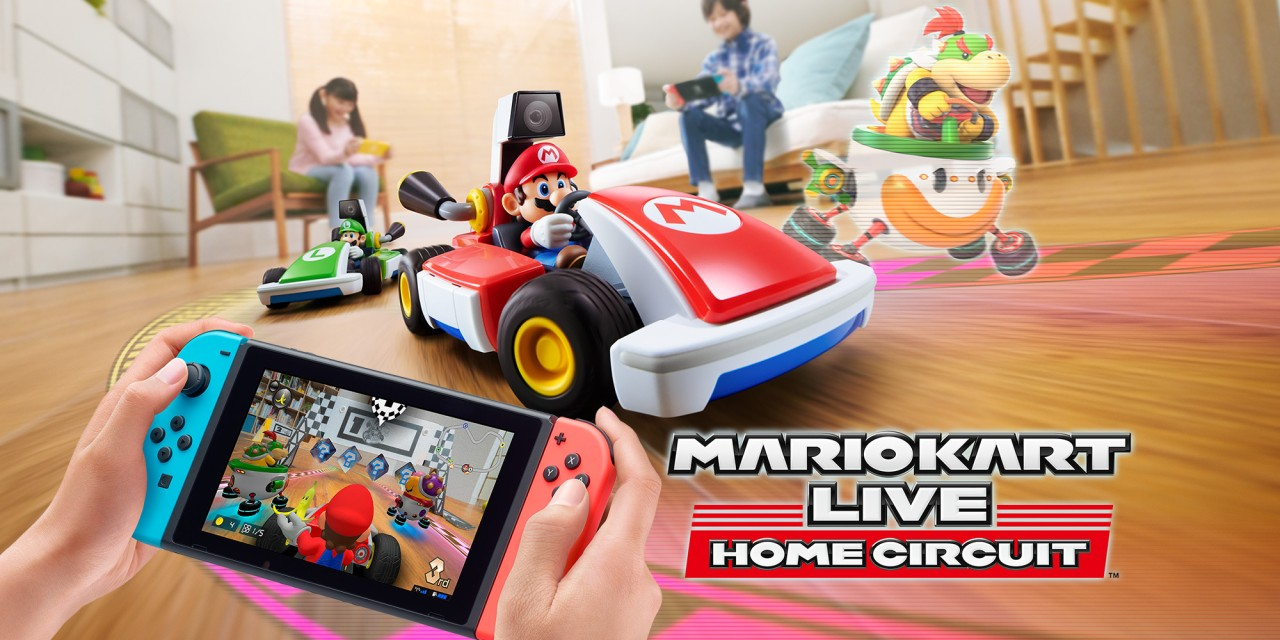
\includegraphics[width=0.8\textwidth]{Images/ExistingGames/MarioKartLive.jpeg}
    \caption{Mario Kart Live poster showing illustrated gameplay.}
    \label{fig:mario_kart_live}
\end{figure}

\subsection{Pokémon Go}
Pokémon Go is another good alternative game example, published and developed by Niantic for iOS and Android. The game was launched in 2016 and quickly became one of the most popular mobile games of all time \citep{grubb_pokemon_2016}. The concept is an extension of the classic Pokémon game found on multiple of Nintendo's handheld devices.

\begin{figure}[H]
    \begin{minipage}{.48\textwidth}
      \centering
      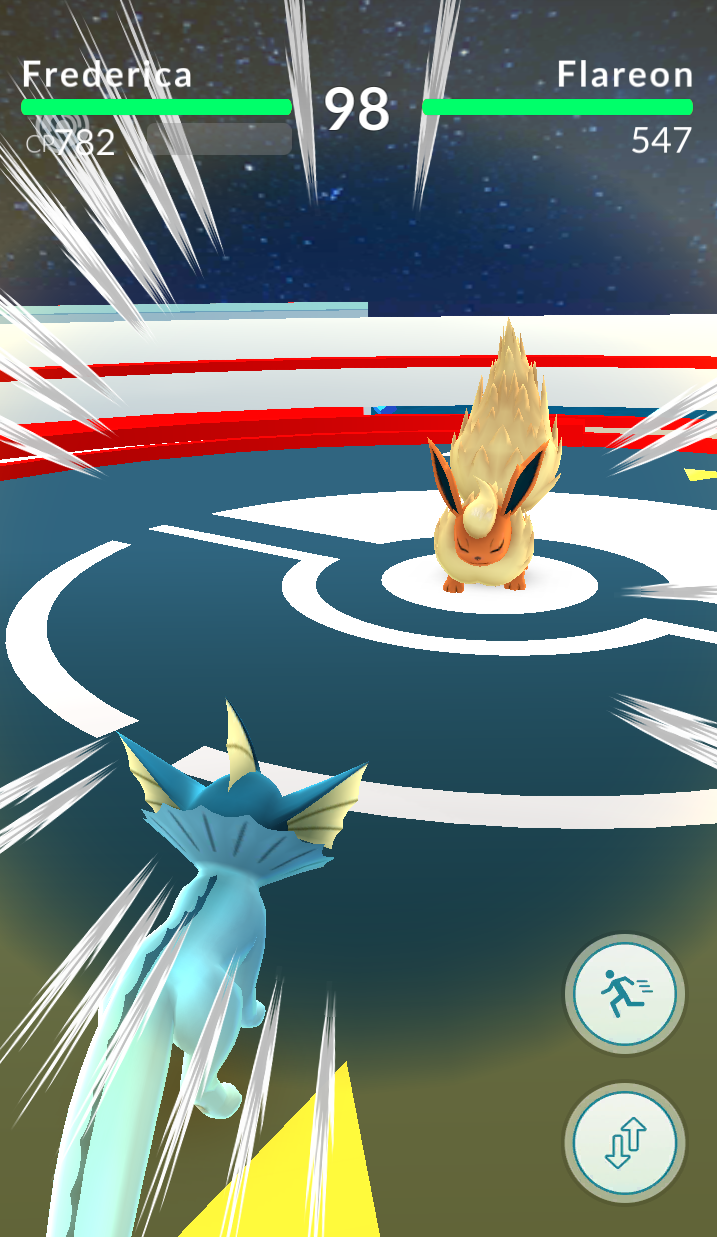
\includegraphics[width=.8\textwidth]{Images/ExistingGames/PokemonGoBattle.png}
      \captionof{figure}{Screenshot of an ongoing battle in Pokémon Go.}
      \label{fig:pokemon_go_battle}
    \end{minipage}
    \hspace{0.5cm}
    \begin{minipage}{.48\textwidth}
      \centering
      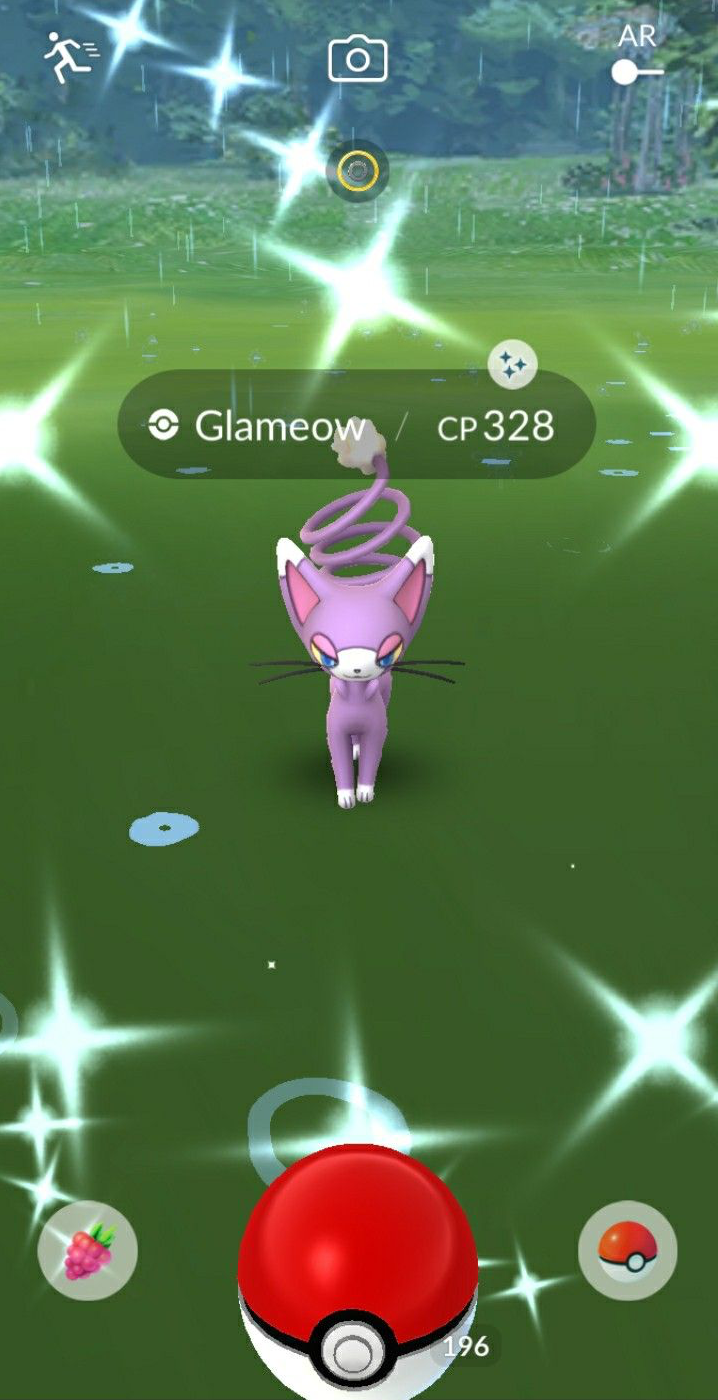
\includegraphics[width=.7\textwidth]{Images/ExistingGames/PokemonGoCatch.png}
      \captionof{figure}{Typical screenshot of gameplay in Pokémon Go.}
      \label{fig:pokemon_go_catch}
    \end{minipage}
\end{figure}

The concept is similar to the previous Pokémon games but utilizes AR and location determination (GPS) to find and catch Pokémons. The player needs to move around in the real world to play the game. Battles between Pokémons (to increase combat points and get prices) can happen at specific places known as Pokémon Gyms. These spots correspond to real-world points of interest (POI) such as parks and tourist attractions \citep{bastow_pokestops_2016}. There are also additional important POI in the game, such as PokéStops and Nests. Figure \ref{fig:pokemon_go_battle} is an in-game screenshot where you can see a typical Pokémon battle, while Figure \ref{fig:pokemon_go_catch} shows a screenshot of gameplay while catching a Pokémon.

The game is an alternative game as it explores uncommon input and output sources such as camera, GPS, and AR. The game is also classified as a pervasive game because the player experience is extended to the real world. A study on \textit{The Pikachu Effect} reveals that the magnitude of Pokémon Go players experience both physical and social benefits from the pervasive game\citep{kaczmarek_pikachu_2017}. Pokémon Go is an excellent example of how alternative games can become very successful.

\subsection{Just Dance Now}
Just Dance Now is an alternative game produced by Ubisoft, launched in 2014 \citep{fandom_just_2020}. The game is an addition to the Just Dance franchise, where the concept is to pick a song from the catalog and follow the moves of the on-screen character, see Figure \ref{fig:just_dance_now_pc}. 

Just Dance Now distinguishes itself from the other games of this type by being more available because it does not require a dedicated gaming console. It can be played using an iOS or Android-based smartphone as the controller and a large screen connected to the internet, such as AppleTV, Chromecast, or a computer \citep{ubisoft_general_2020}. The player's smartphone is used as a movement tracker, and the large screen displays the dance moves they should perform. Multiple players can join the same game and dance together, competing, trying to get the highest score.

\begin{figure}[H]
    \begin{minipage}[t]{.65\textwidth}
        \centering
        
\includegraphics[width=\textwidth]{Images/ExistingGames/JustDanceNow_Pc.png}
        \caption{Just Dance Now screenshot from the computer display.}
        \label{fig:just_dance_now_pc}
    \end{minipage}
    \hspace{0.5cm}
    \begin{minipage}[t]{.35\textwidth}
        \centering
        
\includegraphics[width=0.8\textwidth]{Images/ExistingGames/JustDanceNow_Mobile.png}
        \caption{Just Dance Now screenshot from a smartphone that is used as a movement controller.}
        \label{fig:just_dance_now_mobile}
    \end{minipage}
\end{figure}

The main reason this game can be seen as an alternative game is based on the use of the player’s mobile phone as a movement tracking device, as seen in Figure \ref{fig:just_dance_now_mobile}. Based on the sensors’ measurements in the player’s phone, the game determines whether or not the player is doing the dance moves well.

The interaction form is another reason why this game is an alternative game. The game is an example of a multi-modal exergame, where all players in one game use the same large screen to see the moves they need to perform in order to earn points. A recent study on the use of exergames in physical education in primary schools, revealed that Just Dance Now had positive effects on students performance, engagement, and motivation for physical activity\citep{quintas_psychological_2020}. This concept can also be described as a “Multiplayer On One Screen Entertainment System” (MOOSES), presented in Chapter \ref{chap:what_is_alternative}. 
        
\subsection{Guitar Hero}
Guitar Hero is a series of games initially developed for PlayStation 2 in 2005. The game series later expanded to multiple other game platforms, including Xbox 360 and Nintendo Wii. The game concept is based on simulation and gamification of playing guitar, using a custom-developed guitar controller (see Figure \ref{fig:guitar_hero_controller}). The player tries to match the in-game “notes” with buttons on the guitar controller, resulting in a score coherent with the number of notes hit. Songs available to choose from vary between different games, but generally, they belong to the genre of rock \cite{metacritic_guitar_2020}. Figure \ref{fig:guitar_hero_controller} shows a screenshot example from playing the game in single-player mode. 

One of the categories of alternative game characteristics is input. As per the definition (in Chapter \ref{chap:what_is_alternative}), a game using alternative input sources can be classified as an alternative game. Guitar Hero is a typical example of such a game because it depends on a custom-designed controller for playing. Additionally, the use of gamification as the game genre is another reason why Guitar Hero can be defined as an alternative game. The main concept of the game can be viewed as gamification of playing guitar.

\begin{figure}[H]
    \begin{minipage}{.35\textwidth}
        \centering
        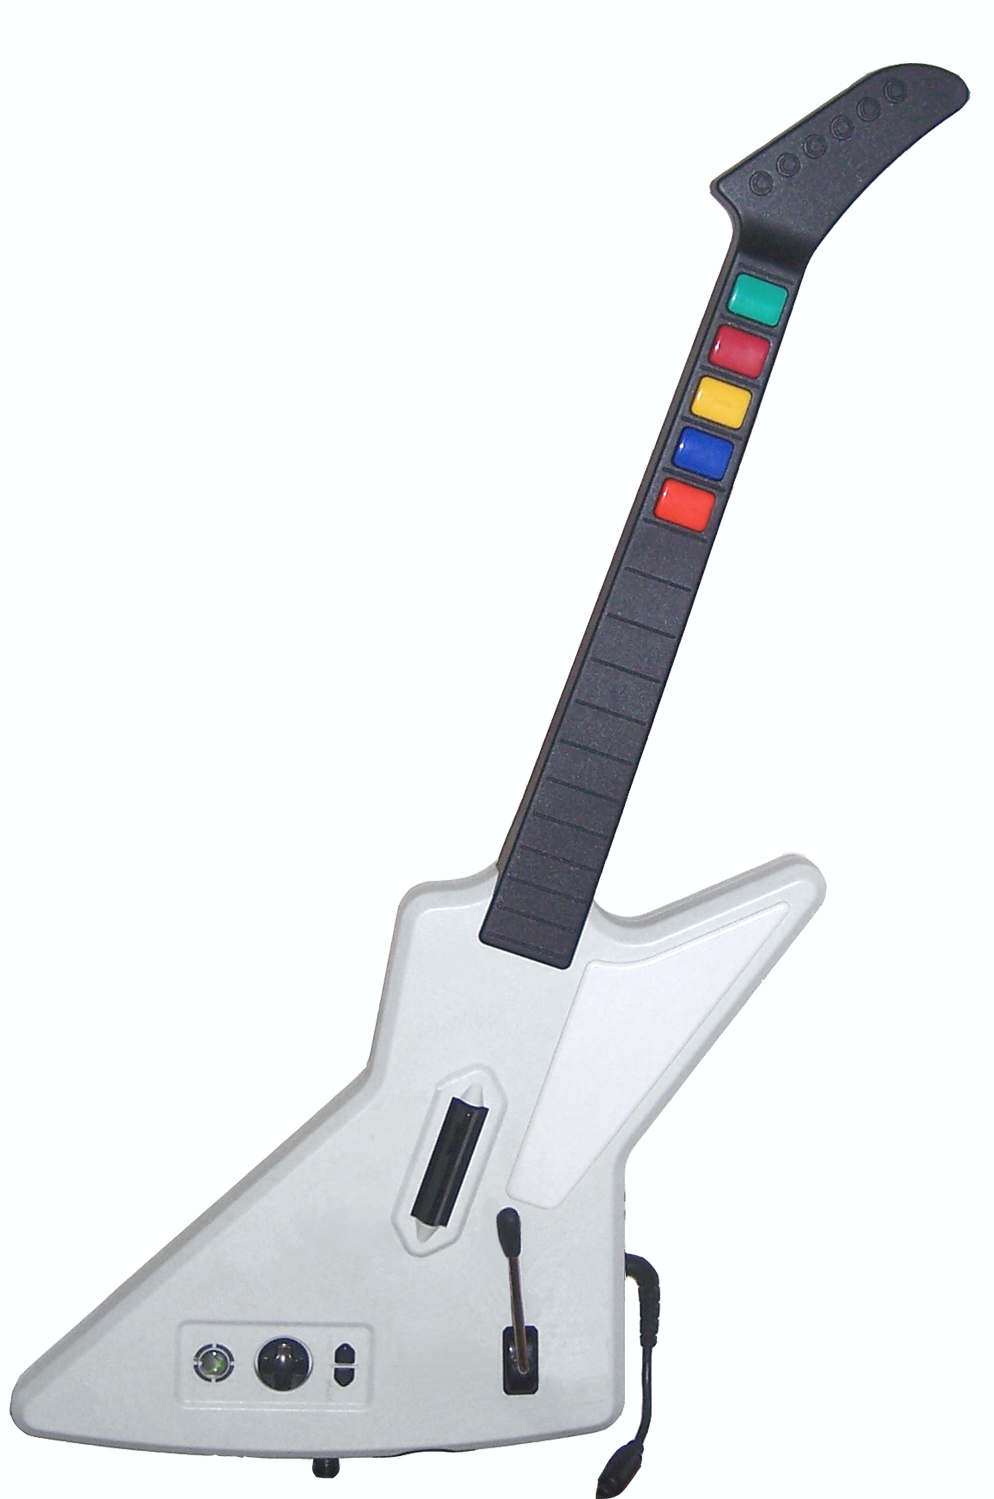
\includegraphics[width=0.9\textwidth]{Images/ExistingGames/GuitarHeroController.png}
        \caption{A Guitar Hero controller.}
        \label{fig:guitar_hero_controller}
    \end{minipage}
    \hspace{0.5cm}
    \begin{minipage}{.65\textwidth}
        \centering
        
\includegraphics[width=0.9\textwidth]{Images/ExistingGames/GuitarHeroScreenshot.jpg}
        \caption{Screenshot from Guitar Hero gameplay.}
        \label{fig:guitar_hero_screenshot}
    \end{minipage}
\end{figure}
        
\subsection{Wii Fit}
Wii Fit is an exercise game (exergame) created by Nintendo that launched in 2007 \citep{imdb_wii_2020}. The game is only available on Nintendo Wii and requires a unique controller in addition to the regular Wii controller. Wii Fit is a collection of minigames that combine the two domains of health and entertainment. The game has four main exercise categories to choose from; strength training, aerobics, yoga, and balance \citep{ign_wii_2008}.

\begin{figure}[H]
    \centering
    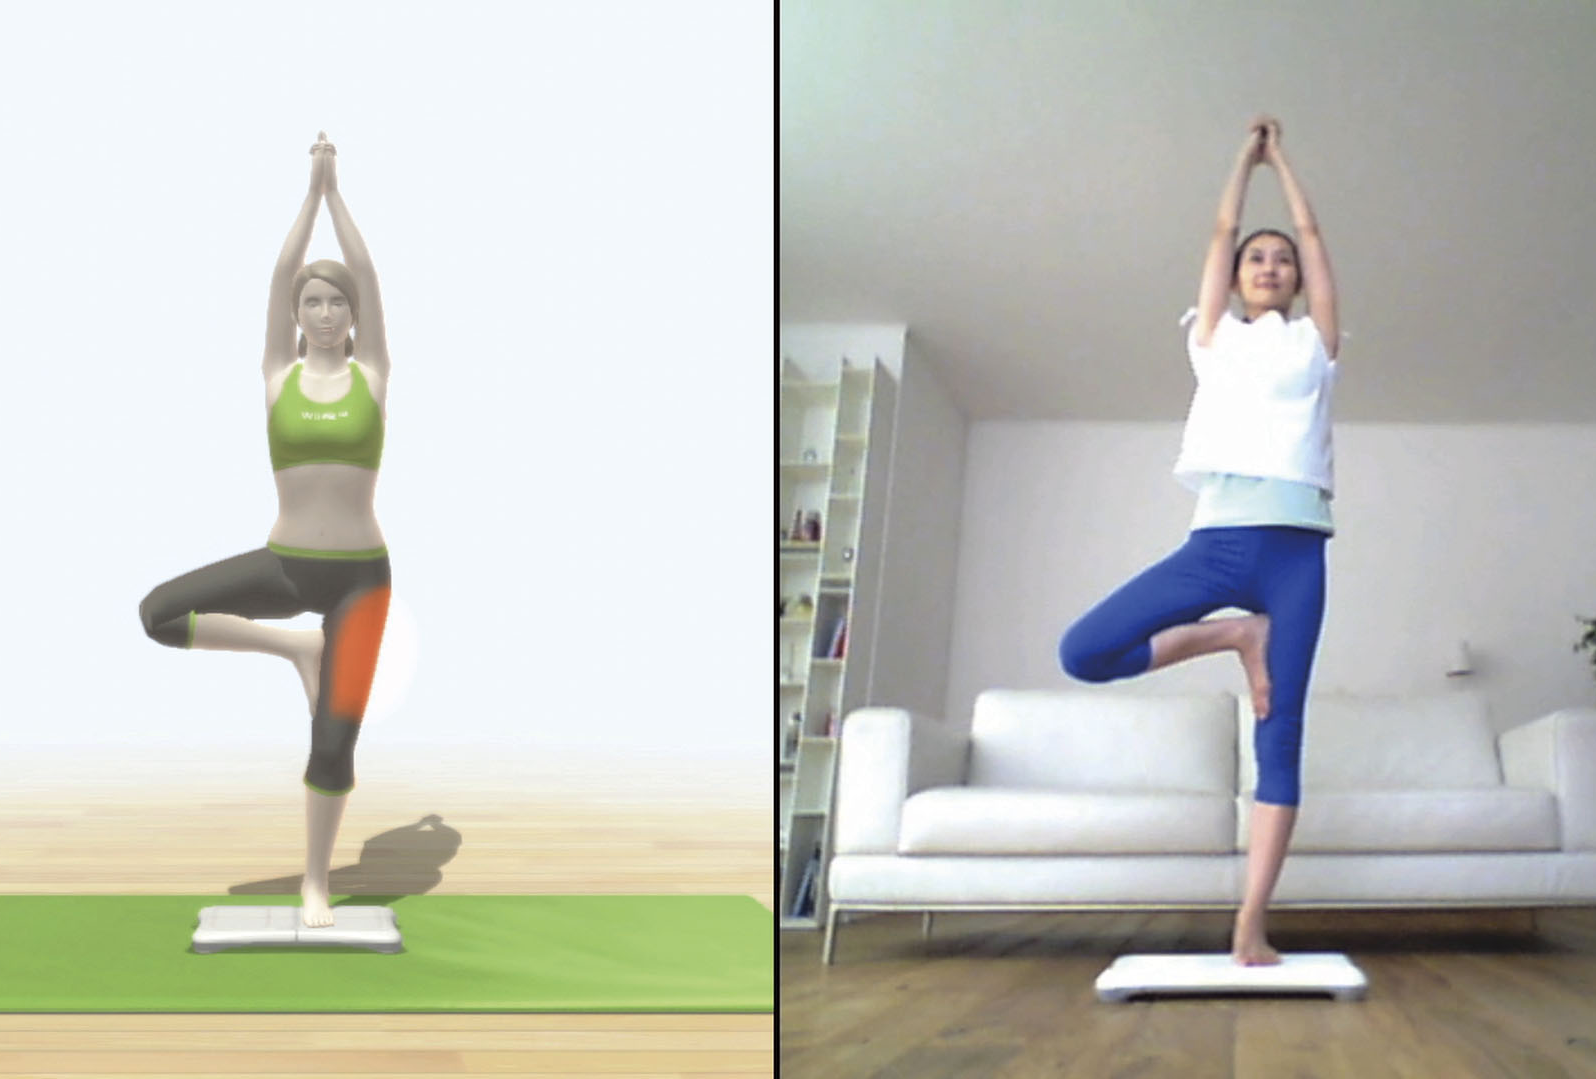
\includegraphics[width=0.75\textwidth]{Images/ExistingGames/WiiFit_Pose.png}
    \caption{A person doing yoga exercise alongside an in-game avatar.}
    \label{fig:wii_fit_pose}
\end{figure}

The additional controller is called the Wii Balance Board \citep{ign_wii_2008} and is one reason this game can be categorized as alternative. The board’s purpose is to track the user's movement and translate it to the user’s in-game avatar, as seen in Figure \ref{fig:wii_fit_pose}. The idea behind the board was drawn from the bathroom weight, and it consists of four weight sensors; one in each corner. The controller connects to the console through Bluetooth, where it calculates the user's movement in real-time \citep{jacquot_how_2010}. Based on the user’s movement, the game gives feedback on how the exercise is going, as seen in Figure \ref{fig:wii_fit_pushup}.

In addition to the alternative input, Wii Fit is also a gamification concept of doing exercise. The game’s goal is to create a fun way of getting in shape from a user’s own home. Nintendo brings a comprehensive set of games that are engaging for the entire family with individual progress so all players can compare themselves against each other.

Wii Fit was originally designed as an interactive health and fitness experience for the general public. However, the benefits of Wii Fit have been studied in many clinical settings, such as in multiple sclerosis patients and stroke patients\citep{tripette_contribution_2017}. A 2011 study of the health and wellness benefits of Wii Fit on university students, revealed a significant change in body mass index, weight, and intrinsic and total motivation for its participants\citep{jacobs_wii_2011}.

\begin{figure}[H]
    \centering
    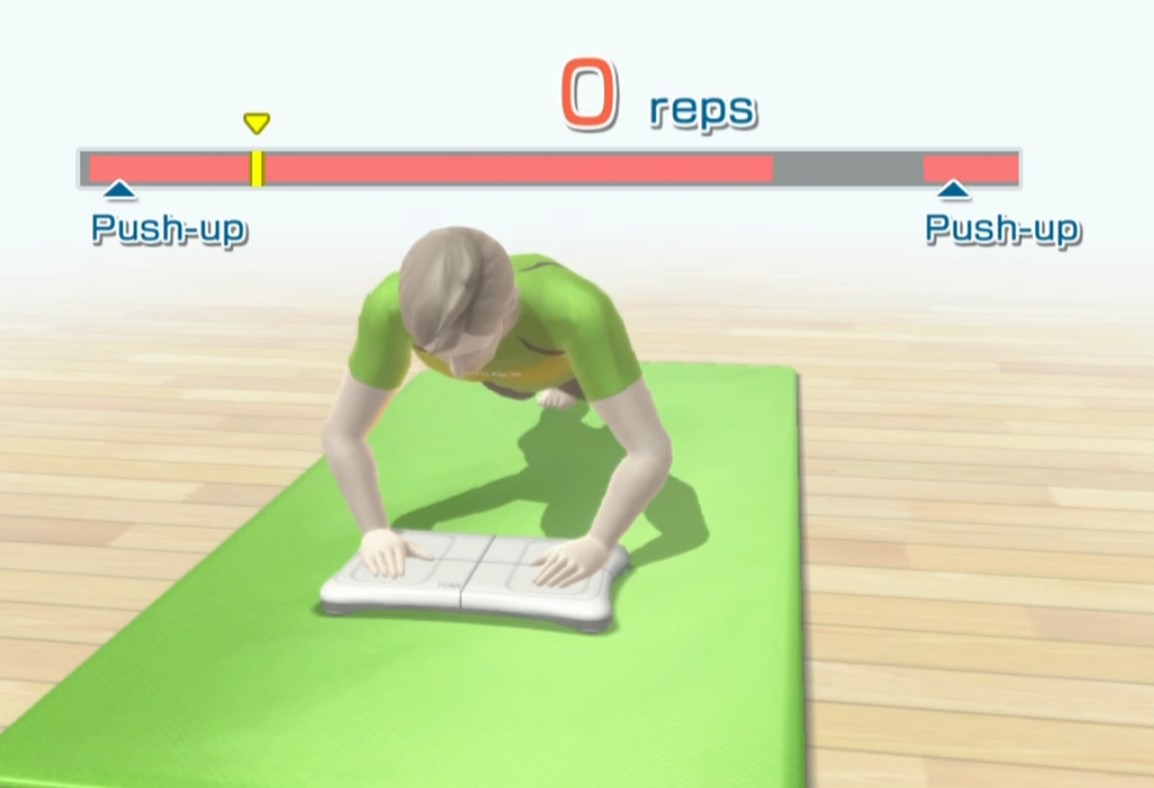
\includegraphics[width=0.75\textwidth]{Images/ExistingGames/WiiFit_Pushup.jpg}
    \caption{Screenshot of the in-game avatar using the board to track push-ups.}
    \label{fig:wii_fit_pushup}
\end{figure}

\subsection{Mosquito Mania}
Mosquito Mania is a game concept developed at NTNU in connection with a music technology bachelor thesis in 2012. The game was developed as an attempt to create a new way of entertaining people by using audio stimulation together with concepts from game development.

The primary purpose of the game is to kill as many mosquitos as possible within 60 seconds. An 8-32 array of speakers is positioned in a circle around the player, emitting mosquito sounds in a 2-dimensional space, as seen in Figure \ref{fig:mosquito_mania_anonym}. The player is then assigned the task to try and kill the mosquitos using a custom made gun-like controller, measuring the direction it is pointed. A microcontroller combined with an accelerometer, compass, and gyroscope is mounted on the controller. Though the game primarily focuses on audio, the game has a dashboard for game statistics and scoreboard (see Figure \ref{fig:mosquito_mania_dashboard})

The game is alternative for multiple reasons. First of all, it uses an alternative input source, i.e., the custom controller for playing. This special controller could by itself contributed to categorize the game as alternative. However, the primary reason for Mosquito Mania to be an alternative game is the unusual approach of using audio as the primary output source. Regular games typically combine sounds and music as a secondary output source in addition to visual feedback. The game concept is unique, and by removing the visual aspect, a new twist is introduced to the game. Even though the game was not developed for any special target groups, it became immensely popular among people with visual impairment \citep{gran-jansen_mosquito_2020}.

\begin{figure}[H]
    \begin{minipage}[t]{.5\textwidth}
        
\includegraphics[width=\textwidth]{Images/ExistingGames/MosquitoMania_anonym.jpg}
        \caption{The player is surrounded by speakers that emit mosquito sounds. The handheld gun is used to aim at the imaginary mosquito to score points.}
        \label{fig:mosquito_mania_anonym}
    \end{minipage}
    \hspace{0.05\textwidth}
    \begin{minipage}[t]{.5\textwidth}
        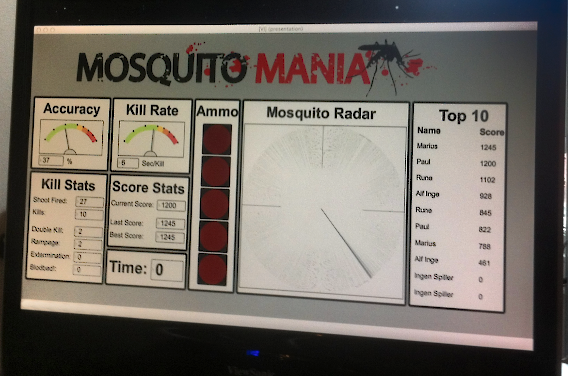
\includegraphics[width=0.87\textwidth]{Images/ExistingGames/MosquitoMania_Dashboard.png}
        \caption{The game’s dashboard shows game statistics and a top 10 scoreboard.}
        \label{fig:mosquito_mania_dashboard}
    \end{minipage}
\end{figure}

\biblio % Needed for referencing to working when compiling individual subfiles - Do not remove
\end{document}
\clearpage

\documentclass[../Main.tex]{subfiles}
\begin{document}

\section{Comparison of Existing Alternative Games}
\label{chap:comparison_of_existing}
To more compare the alternative aspects of all the games mentioned in this chapter, the model based on the categories of characteristics presented in Chapter \ref{chap:what_is_alternative} has been used. It gives a quick overview of how the game differs and presents concrete characteristics for all the games in each of the six categories. The model in Table \ref{tab:existing_games} is a simplified version of the complete model found in Appendix \ref{appendix:complete_model}. The rows not used have been omitted for readability. A complete version can be found in Appendix \ref{appendix:complete_model}. 

\begin{table}[H]
    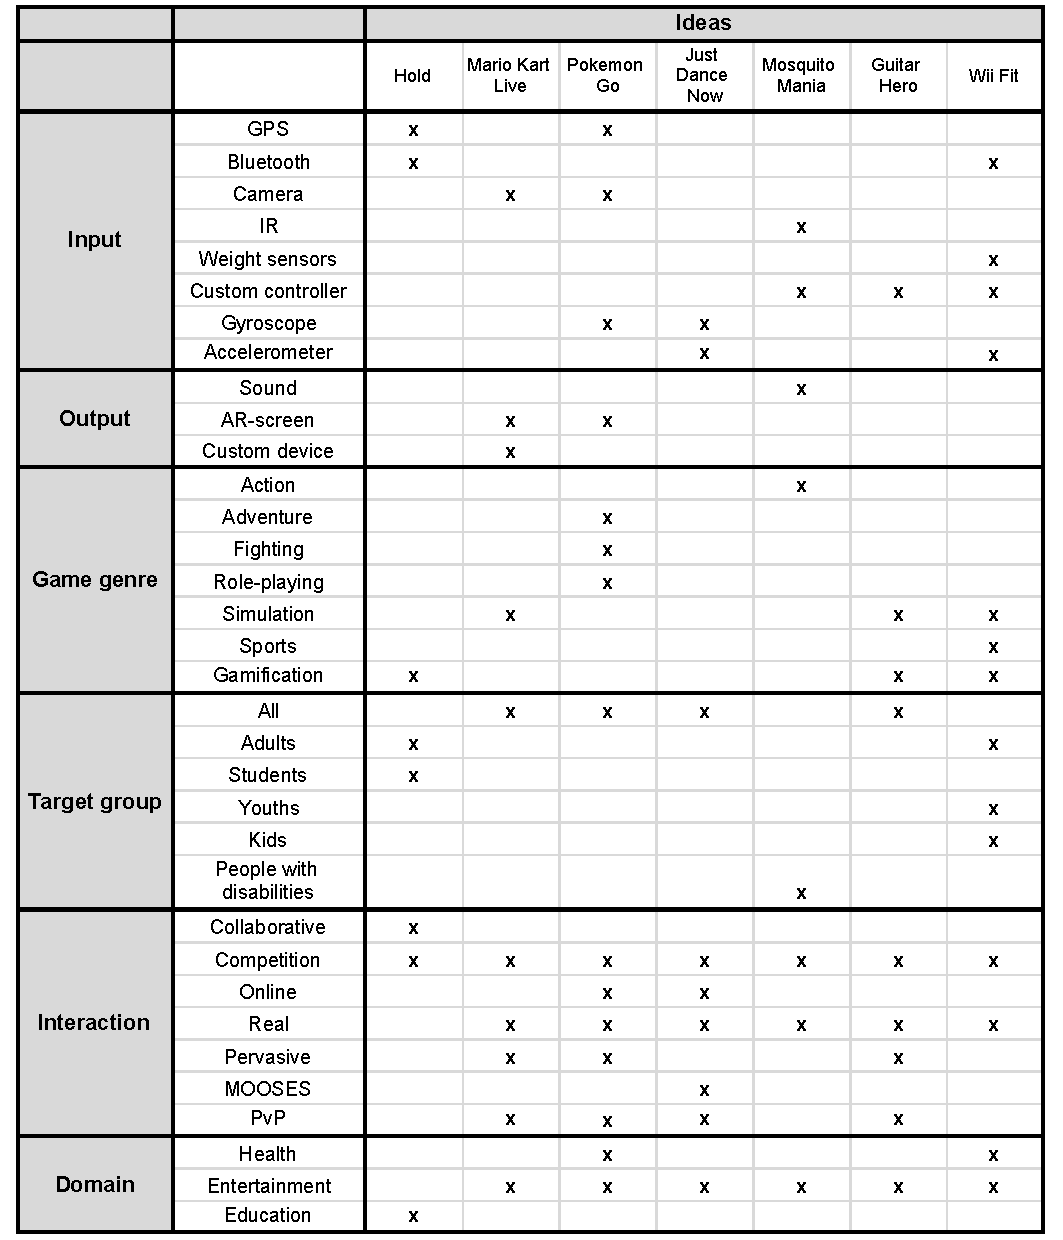
\includegraphics[width=1\textwidth]{Images/Models/ExistingGames.pdf}
    \caption{Existing alternative games characteristics}
    \label{tab:existing_games}
\end{table}

\subsection{Analysis of Input}
The first section of the model shows a wide range of \textit{input} types used in the games. The variation of input types is likely to come from the platform in use. Most mobile phones used today include various input sensors that can be used to develop alternative game concepts. GPS, Bluetooth, gyroscope are examples of such sensors.

The games Hold, Pokémon Go, and Just Dance Now are totally or partially developed for mobile platforms. Hold and Pokémon Go uses the device’s GPS to use the context of the player’s location in the game. The location-aware feature creates a better in-game experience, and players are forced to move to unlock certain features. Pokémon Go and Just Dance Now both take advantage of the phone’s gyroscope. The gyroscope can detect rotation, and for these games, the rotation tells the game how the mobile device is positioned in the real world. Just Dance Now also uses the accelerometer to track the player’s movement while dancing. The use of both gyroscope and accelerometer determines if the player is hitting the right moves at the right time, which gives better accuracy and better player-experience in this alternative game.

Guitar Hero, Wii Fit, and Mosquito Mania all use custom controllers. In the early days of games, many games used to have custom controllers \citep{overmars_brief_2012}. However, this was not fortunate for the user because it forced them to buy new controllers for each game. Nowadays, custom controllers are rare because games are often produced for specific consoles that already have an official controller. Furthermore, non-custom controllers can cause a poor user experience because they might not have an optimal or logical design. The Guitar Hero, Wii Fit, and Mosquito Mania are examples of games not suited for the standard console controller. In these games, it makes sense to use a custom controller more fit for the game's purpose. An unusual controller used as input is a classic example of an alternative game.


\subsection{Analysis of Output}
The second section of the model looks at the alternative use of \textit{output} in games. Even though today’s games often use sound effects and music, this does not make them alternative. Mosquito Mania uses sound in a more alternative scenario, as this is the only output in the game. The game focuses on the player's ability to sense the sound's direction, which is an alternative way of challenging the player's hearing instead of the eyesight.

Furthermore, Pokémon Go and Mario Kart Live use the camera as an input to produce an Augmented Reality (AR) output. AR technology is alternative in games because projecting artificial objects onto the real world is based on interpreted input. In both games, players use a handheld device. AR in mobile devices is available for the consumer considering the technology within the device. However, mobile devices do not create an immersive gaming experience compared to an AR headset.


\subsection{Analysis of Game Genre}
A selection of \textit{game genres} is listed in the third section of the table. These game genres themself do not make games alternative. However, they do tell something about what type of game it is. There is one exception to this: gamification. Gamification is alternative because it gamifies activities and tasks to make it fun and engaging while motivating the player. Hold, Guitar Hero, and Wii Fit are all gamification of activities or issues. Hold gamifies and rewards players for putting the phone down, Guitar Hero gamifies playing the guitar, and Wii Fit gamifies and motivates working out. Furthermore, games can also be classified within multiple genres, making the game more alternative. However, this is not implied.

\subsection{Analysis of Target Group}
The identified \textit{target groups} can be found in the fourth section of Table \ref{tab:existing_games}. All games have one or more dedicated target groups, corresponding to everyone or a distinguished set of users. The target groups might overlap or intersect; for instance, students and young adults intersect. Mario Kart Live, Just Dance Now, and Guitar Hero are some of the games that can be played by most people. These games might, however, address a younger crowd. Mosquito Mania is a game that can be played by most people, however, as an audio game the game can also be played by people with visual impairment.

\subsection{Analysis of Interaction}
The fifth section of the table displays the types of \textit{interactions} that have been identified in the existing games studied in Chapter \ref{chap:existing_games}. Interaction types can be found in all ordinary games and do not imply that a game is alternative. However, the type of interaction can be alternative in how player interaction is accomplished. All of the seven games use a combination of interaction methods, and all games include some degree of interaction through competition. Competition can be accomplished in numerous ways in real-time or by a scoreboard. Just Dance Now offers, like many other games, different player modes. Players can compete online in real-time, PvP, multimodal, or get high scores for the global scoreboard. These gameplay variations make the game very flexible, and players can play in whatever way they want. The other games offer similar but not so extensive features as Just Dance Now. Mario Kart Live, Pokémon Go, and Guitar Hero all include the competitive feature of PvP interaction. In these games, players communicate in the real world, but the gameplay happens in the virtual world.

Hold is the only game that includes a collaborative mode. Players can connect their device with their friends’ to boost points; if one player quits, the player will not only lose his or her focus but also stop the boosting for the collaborating players. This interaction feature is likely to strengthen the player’s motivation for not using their phones.
 

\subsection{Analysis of Domain}
The sixth and last section of the model displays the \textit{domain} of the games. Traditionally speaking, games often belong to the domain of entertainment. Some alternative games have an alternative area of use and therefore touches within one or more domains. The exercise game Wii Fit is directly connected to the domain of physical health. Pokémon Go also exploits the benefits of physical health from having players move around. The exploiting of other domains than entertainment makes these games more alternative. On the other hand, Hold is not like traditional games and does not classify under the entertainment domain. Its target group is students and is therefore used indirectly in the domain of education.

\subsection{Summary}
This chapter has focused on showcasing multiple different and typical examples of alternative games (based on our definition presented in Chapter \ref{chap:what_is_alternative}). The examples have been shortly described and compared with each other to highlight their differences. A table with the characteristics of each game has been presented and analyzed. The next chapter will shift the focus from the concept of alternative games to the technical aspect of the field. 

\biblio % Needed for referencing to working when compiling individual subfiles - Do not remove
\end{document}
\clearpage

\documentclass[../Main.tex]{subfiles}
\begin{document}

\section{Technology Review}
\label{chap:technology_review}

\subsection{Diversity in Alternative Game Technology}
% Probably should wrap this figure
\begin{figure}[H]
    
\includegraphics[width=0.8\textwidth]{Images/TechnologyReview/SingstarController.jpg}
    \centering
    \caption{Singstar controller}
    \label{fig:singstar_controller}
\end{figure}

\subsection{Mobile Application Development Tools}
\begin{figure}[H]
    
\includegraphics[width=0.8\textwidth]{Images/TechnologyReview/ARGlasses.jpeg}
    \centering
    \caption{Ar glasses}
    \label{fig:ar}
\end{figure}

\begin{figure}[H]
    \begin{minipage}[t]{.55\textwidth}
         
\includegraphics[width=0.84\textwidth]{Images/TechnologyReview/OculusQuest.jpg}
        \centering
        \caption{Oculus quest}
        \label{fig:oculus}
    \end{minipage}
    \hspace{0.05\textwidth}
    \begin{minipage}[t]{.45\textwidth}
        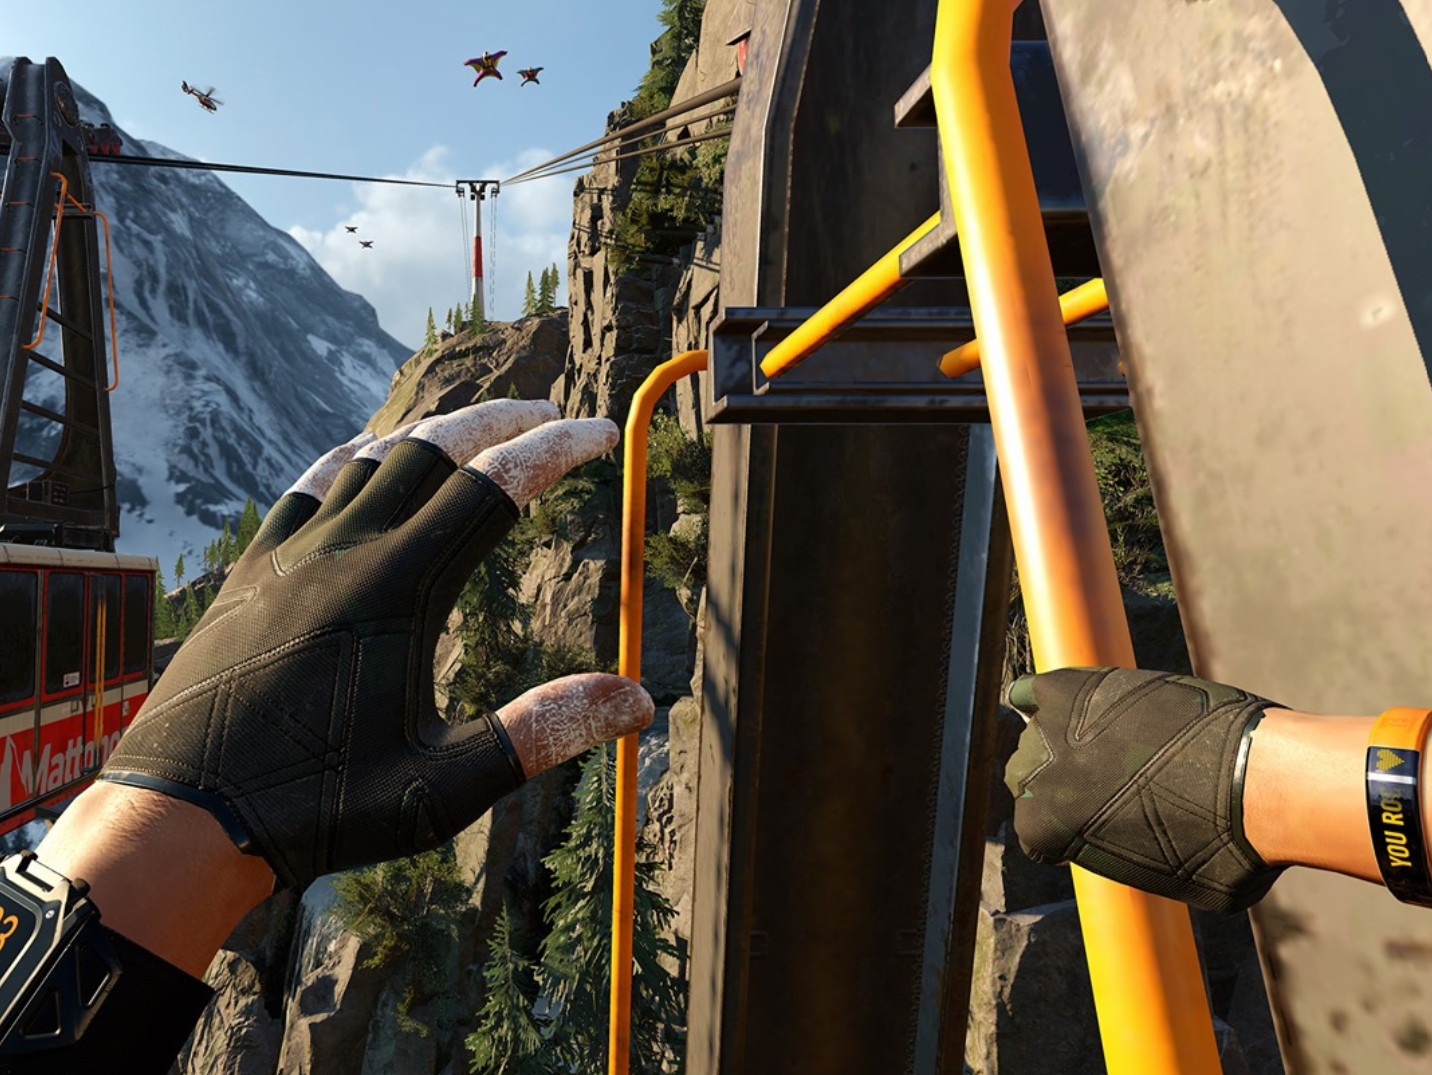
\includegraphics[width=0.8\textwidth]{Images/TechnologyReview/TheClimbOculus.jpg}
        \centering
        \caption{The climp}
        \label{fig:theclimb}
    \end{minipage}
\end{figure}

\subsubsection{Native Solutions}
\subsubsection{Cross-platform solution}
\subsubsection{Choosing Between Native and Cross-platform}

\subsection{Data Solutions}
\subsubsection{Backend as a Service (BaaS)}
\subsubsection{Custom API}
\subsubsection{Choosing between BaaS and a Custom API}

\subsection{Summary}

\biblio % Needed for referencing to working when compiling individual subfiles - Do not remove
\end{document}
\clearpage